\documentclass{article}
\usepackage[a6paper,
            total={105mm, 148mm},
            margin=30pt,
            twoside % Tillåter olika placering av sidnummer på udda och jämna sidor
]{geometry}
\usepackage{fancyhdr}
\usepackage{parselines}
\usepackage{float}
\usepackage{graphicx}
\usepackage[absolute,overlay]{textpos}  % Package for absolute positioning
\usepackage{atbegshi}

\usepackage{imakeidx} % Registret
\usepackage{background} % Gråa Krusidull-E:et och alla bilder
\usepackage{ifoddpage} % Gråa Krudidull-E:et på udda sidor


\usepackage[absolute,overlay]{textpos} % For images
% Set the positioning units to centimeters
\setlength{\TPHorizModule}{1cm}
\setlength{\TPVertModule}{1cm}


\usepackage{xcolor} % BARA I BÖRJAN FÖR MARKERING TILL OSS SJÄLVA


% Insert transparent background to remove background
\newcommand{\noBackground}{
  \backgroundsetup{
    scale=0.65,
    opacity=0.0,
    angle=0,
    color=black,
    vshift=-130,
    hshift=50,
    contents={
\includegraphics[width=\paperwidth]{./bilder/no_background.png}}
  }
}

% Normal background setup for odd pages
\backgroundsetup{
  scale=0.65,
  opacity=0.075,
  angle=0,
  color=black,
  vshift=-130,
  hshift=50,
  contents={%
    \checkoddpage
    \ifoddpage
      
\includegraphics[width=\paperwidth]{./bilder/large_E.png}
    \else
      %
\includegraphics[width=\paperwidth]{../bilder/VarumarkesBildServlet.jpg}
      \noBackground
    \fi
  }
}


\newcommand{\custombackground}[1]{
  \backgroundsetup{
    scale=0.65,
    opacity=0.0,
    angle=0,
    color=black,
    vshift=-130,
    hshift=50,
    contents={\includegraphics[width=\paperwidth]{#1}}
  }
}


\newcommand{\resetBackground}{
  \backgroundsetup{
    scale=0.65,
    opacity=0.075,
    angle=0,
    color=black,
    vshift=-130,
    hshift=50,
    contents={%
      \checkoddpage
      \ifoddpage
        
\includegraphics[width=\paperwidth]{./bilder/large_E.png}
      \else
        %
\includegraphics[width=\paperwidth]{../bilder/VarumarkesBildServlet.jpg}
      \fi
    }
  }
}



% Disable indentation for the whole document
\setlength{\parindent}{0pt}


% Use fontspec with XeLaTeX or LuaLaTeX to load system fonts
\usepackage{fontspec}

% Set up the subsection font to Lucida Sans Unicode
\usepackage{titlesec}
\titleformat{\subsection}
  {\normalfont\fontsize{12pt}{10pt}\selectfont\fontspec{Lucida Sans Unicode}} % Adjust the size if needed
  {\thesubsection}{1em}{}

% Adjust vertical spacing around subsection titles
\titlespacing{\subsection}
{0pt}                % Left margin
{0.5ex plus .2ex}    % Space before subsection title (adjust as needed)
{0.5ex plus .2ex}    % Space after subsection title (adjust to decrease space after)

% Adjust footskip to add space below the footer
% \setlength{\footskip}{20pt} % Flyttar upp footern lite ########################################## Denna funkar inte riktigt som jag trodde. Jag vill flytta upp sidnumret lite mer
\setlength{\textheight}{120mm}


% Define the page style
\fancypagestyle{main}{
  \fancyhf{} % clear all header and footer fields
  \fancyhead[RO]{\hfill \footnotesize\scshape\leftmark \hfill}
  % \fancyfoot[LE,RO]{\thepage}

  % Adjust the page number position
  % Set page number closer to the edge by increasing the right margin
  \fancyfoot[LE]{\hspace{-17pt}\thepage} % Flytta ut sidnummer jämna sidor
  \fancyfoot[RO]{\thepage\hspace{-17pt}} % Flytta ut sidnummer udda sidor

  % Ta bort linje under/över header och footer
  \renewcommand{\headrulewidth}{0 pt}
  \renewcommand{\footrulewidth}{0 pt}

  % Använder footnote for 'visste du att'
  \renewcommand{\footnoterule}{}
  \renewcommand{\thefootnote}{}
}

% Set up textblock package to work with A6 paper
\setlength{\TPHorizModule}{1mm}  % Set horizontal units to mm
\setlength{\TPVertModule}{1mm}   % Set vertical units to mm

% Define the custom command to place text at the bottom of the page
\newcommand{\vissteduatt}[1]{%
    \begin{textblock*}{100mm}(12mm,137mm) % Adjust (2.5mm, 140mm) to position text
        \raggedright
        {\footnotesize{\textit{#1}}}
    \end{textblock*}
    \newpage % Ensures that the text appears only on the current page
}


% Define the custom command for small font and italics
\newcommand{\songinfo}[1]{%
  \textit{\small #1 \\}%
}









% DETTA SÄTTET ATT GÖRA REGISTER FUNGERAR BRA OCH ÄR LÄTT MEN DET BLIR INTE LIKA SNYGGT UTAN PUNKTERNA



% HITTA ETT SÄTT ATT GÖRA ETT SNYGGARE REGISTER INNAN VI FORTSÄTTER ATT LÄGGA TILL LÅTAR ETC. 
\makeindex[ % Alfabetiskt register
  name=alfa,
  columns=1,
  title=Alfabetiskt Register,
  intoc,
  options = {-s styleAlfa.ist}
]
\makeindex[ % Analfabetiskt register -- början av sången
  name=anfa,
  columns=1,
  title=Analfabetiskt Register,
  intoc,
  options = {-s styleAlfa.ist}
]


\begin{document}

% Apply the 'main' page style
\pagestyle{main}

% Title and empty page without header/footer
\NoBgThispage
\begin{titlepage}
    \centering
    \vspace{1cm}
    {\fontsize{18}{18}\selectfont E-sektionens sångbok}\\
    \vspace{0.2cm}
    {\fontsize{30}{30}\textbf{Komponenten}}\\
    \vspace{0.2cm}
    {\fontsize{15}{15}\textit{2:a upplagan}}
    \thispagestyle{empty}

    \begin{figure}[H]
      \centering
      
\includegraphics[width=1\textwidth]{./bilder/large_E.png}
    \end{figure}

\end{titlepage}


\newpage

% 
Borra ett hål i pärmen här för att fästa din penna: {\Huge $\bullet$}

\subsubsection*{Konsten att sjunga!}
Att sjunga är verkligen något av det roligaste som finns\dots


Jag vet inte riktigt vad vi vill skriva här\dots

Att sjunga är kul\dots



Morris Thånell BME19 och Elin Helmersson E21\\
Sångbokskommittén 2024



\newpage

Tack till de som hjälpt oss med boken!

\newpage

\begin{center}
    \textbf{Viktig information}
\end{center}

% \backgroundsetup{ 
%   scale=0.36,
%   opacity=1,
%   angle=0,
%   color=black,
%   vshift=300,
%   hshift=151,
%   contents={
\includegraphics[width=\paperwidth]{./bilder/profilbild.png}}
% }

\begin{textblock*}{6cm}(6cm,1.5cm) % {block width}(x-coordinate, y-coordinate)
  
\includegraphics[width=3.5cm]{./bilder/profilbild_stor.png} % Adjust the image size as needed
\end{textblock*}
\begin{parse lines}[\noindent]{#1\\}
    Ägare:

    Sektion(?):
    
    Inskrivningsår:
    
    Födelsedatum:



    Lämna tillbaka mig till den här adressen:


    Hittelön:
    Om jag inte varit teknolog hade jag varit:
    Om jag fick välja nollningstema:


    Favoritmat:
    Favoritband:
    Favorit
    Bästa 
    Favoritintegral:
    
    .... Rita eller klistra en bild

\end{parse lines}

\newpage

% \subsubsection*{Innehållsförteckning}
\tableofcontents

\newpage
\begin{center}
  \vspace*{1.5cm}
  {\fontsize{20}{20}\textbf{Vett och etikett}}\\
  \vspace{0.7cm}
  {\fontsize{12}{12}\textit{Om den pryde själv får välja}}
\end{center}
\addtocwithheader{Vett och etikett}  % Add entry to TOC and set header
\noBackground
\newpage

\subsubsection*{KLÄDKOD}
För att underlätta förmedlingen av vem som ska ha på sig vad använder vi oss av följande namn.

\textbf{Truls}: Manlig teknolog\\
\textbf{Trula}: Kvinnlig teknolog\\
\textbf{Trelsa}: För hen som inte vill identifiera sig med någon av ovanstående.\\

\subsubsection*{Högtidsdräkt - Militäruniform och folkdräkt}

\textbf{Truls}: Militäruniform, folkdräkt eller frack\\
\textbf{Trula}: Militäruniform, folkdräkt eller balklädding\\
\textbf{Trelsa}: Se Truls/Trula\\

\subsubsection*{Civil högtidsdräkt}

\textbf{Truls}: Frack, vit skjorta, vit fluga\\
\textbf{Trula}: Balklädding\\
\textbf{Trelsa}: Se Truls/Trula\\

\subsubsection*{Smoking}
\textbf{Truls}: Smoking, vit skjorta, svart fluga\\
\textbf{Trula}: Lång klänning, dock behöver den inte vara lika elegant som en Balklädding. Tänk festligt.
\textbf{Trelsa}: Se Truls/Trula\\

\subsubsection*{Mörk kostym}
\textbf{Truls}: Mörkblå, mörkgrå eller svart kostym. Vit skjorta med sidenslips eller fluga i valfri färg.\\
\textbf{Trula}: En finare känning, men även byxdress elelr halvlång kjol med jacka går bra.\\
\textbf{Trelsa}: Se Truls/Trula\\

\subsubsection*{Kavaj}
Ibland även kallad bruten elelr udda kavaj.\\
\textbf{Truls}: Kavaj och ett par finare byxor (dock inte kostymbyxor), skjorta i valfri färg. Fluga eller slips kan vara trevligt!\\
\textbf{Trula}: Cocktailklänning, kjol eller dress.\\
\textbf{Trelsa}: Se Truls/Trula\\

\subsubsection*{Mörk kostym}
\textbf{Truls}: Ouvve \textbf{Hur vill vi stava ouvve/ovve i boken?}\\
\textbf{Trula}: Ouvve\\
\textbf{Trelsa}: Se Truls/Trula\\


\subsubsection*{KLÄDKOD version 2?}
Kåren har ett annat upplägg på hur de visar klädkoderna. Vill vi göra som dem?
\\

Exempel (kopierat från kårens bok)

\subsubsection*{Högtidsdräkt/högtidsklädsel}
För honom är frack lämplig. 
En fin golvlång klänning gäller för henne 
- ett bra material och ett tjusigt sntit ska det vara på den. 
Vill man bära handskar till klänningen går det bra, 
men glöm inte att ta av dem när du äter. 
Både han och hon kan istälet bära hembygdsdräkt eller militär högtidsdräkt.


\newpage

\subsubsection*{ETIKETT}

\subsubsection*{Vid bordet}
Han har sin bordsdam till höger om sig och hon har sin bordsherre till vänster.
Herren drar ut stolen till höger för att hjälpa sin bordsdam till bords eller från bordet. 


\textbf{Denna visste du att måste nog skrivas om eller ändra storleken på all text i boken. Vi ahr lite större text än i gamla komponenten vilket göra att vi inte får plats med riktigt lika mycket text på varje sida....}

\vissteduatt{Visste du att bordsherre och bordsdam är bordsplaceringsbenämningar\\ som avser att underlätta sittningsförfarande och är helt könsneutralt?}

% \input{kapitel/01-sånger.tex}

% \begin{center}
    \vspace*{1.5cm}
    {\fontsize{20}{20}\textbf{E-sektionens visor}}\\
    \vspace{0.7cm}
    {\fontsize{12}{12}\textit{Om E:aren själv får välja}}  
\end{center}
\addtocwithheader{E-sektionens visor}  % Add entry to TOC and set header
\noBackground

\newpage
\resetBackground


\subsection*{E-sektionens Kampvisa I}
\index[alfa]{E-sektionens Kampvisa I}
\index[anfa]{Det sprakar så glatt i vårt hår}
\songinfo{Mel: Stars and Stripe \textbf{OSÄKER MELODI?}}

\begin{parse lines}[\noindent]{#1\\}
    Det sprakar så glatt i vårt hår
    ur öronen sprutar det gnistor
    och strömmarna i våra tår
    laddar upp oss när vi går.

    I hjärnan vi har resistans
    och ström genom motstånd ger en spänning
    och spänning det vill vi ju ha.
    Vi går på E! Vi går på E!
    Vi går på Elström!

\end{parse lines}


\subsection*{E-sektionens Kampvisa II} 
\index[alfa]{E-sektionens Kampvisa II}
\index[anfa]{E, E, E vill vi se}
\songinfo{Mel: Trink, trink, brüderlein trink}

\begin{parse lines}[\noindent]{#1\\}
    E, E, E vill vi se
    E är det bästa där é
    E, E, E vill vi se
    E får oss alla att le!
    Spänning där é i vär erotik
    vi kör med medicin och teknik.
    Spänning där é i vår erotik
    vi kör med elektroteknik

\end{parse lines}

\vissteduatt{Visste du att E-sektionen har sjukt många kampvisor? ELLER \\Visste dua tt Kampvisa II reviderades för att innefatta båda utbildningarna på E-sektionen?}

% \newpage

\subsection*{E-sektionens Kampvisa III} 
\index[alfa]{E-sektionens Kampvisa III}
\index[anfa]{Vi é elteknister ifrån LTH}
\songinfo{Mel: Vi äro musikanter}

\begin{parse lines}[\noindent]{#1\\}
    Vi é elteknister ifrån LTH.
    Hos oss finns inga brister och dé é ju som så.

    (Att) Vi kan lödda, räkna, dricka, bränna sprit.
    Upp till Lophtet, kom så går vi dit!

    Vi kan räkna tangens, sinus, derivera, integraler.
    Vi kan koda singelchip och mata våran pic.

    Ett in, noll ut, rulla kabel, heja vit!
    Vi vill att just du skall komma hit.

    Hoppa i din vita overall och börja gå.
    Elteknik på LTH det bästa du kan få!

\end{parse lines}


\subsection*{E-sektionens Kampvisa IV} 
\index[alfa]{E-sektionens Kampvisa IV}
\index[anfa]{Vi vill ha mera E}
\songinfo{Mel: Mera mål}

\begin{parse lines}[\noindent]{#1\\}
    Vi vill ha mera E, flera E
    Å E det kommer ni att se
    Vi vill ha mera E, mycket mer
    Se upp här kommer vi från E

\end{parse lines}

\vissteduatt{Visste du att E-sektionen är den äldsta sektionen på LTH?}

\newpage


\subsection*{E-sektionens Kampvisa V} 
\index[alfa]{E-sektionens Kampvisa V}
\index[anfa]{Alla vi på E-sek klappar nu} % VILL VI HA DENNA ENS?
\songinfo{Mel: Klappa händerna}

\begin{parse lines}[\noindent]{#1\\}
    //: Alla vi som går på E-sek klappar nu ://

\end{parse lines}


\subsection*{E-sektionens Kampvisa VI} 
\index[alfa]{E-sektionens Kampvisa VI}
\index[anfa]{Vi går på E-sek}
\songinfo{Mel: Man ska ha husvagn}

\begin{parse lines}[\noindent]{#1\\}
    Vi går på E-sek, och vi har spänning så som få
    Vi går på E-sek, äldst och bäst på LTH
    Vi går på E-sek, vår färg är vit, Elektrovit!
    Vi går på E-sek, LTH:s elit!

\end{parse lines}


\begin{textblock*}{3cm}(3.5cm,8.9cm) % {width}(x, y)
    
\includegraphics[width=4.5cm]{./bilder/Transistorer.png}
\end{textblock*}

\vissteduatt{Visste du att några kampvisor blivit reviderade i efterhand?}


\newpage

\subsection*{E-sektionens Kampvisa VII} 
\index[alfa]{E-sektionens Kampvisa VII}
\index[anfa]{E-sek på LTH} 
\songinfo{Mel: Anton aus Tirol \\ Text: Sebastian Elm (E12), Kewin Erichsen (E11)}

\begin{parse lines}[\noindent]{#1\\}
    ||: E-sek, E-sek, E-sek på LTH :||
    Vi slajdar in,
    med grym entré
    För det är vi som går på E!
    Vi lyser upp med bra manér,
    tänder gnistan inom er
    Det är eliten som ni ser!

    Är du för klen?
    De' e ingen kris
    Det fixar vi med dialys!
    När ni sedan vaknat opp,
    är vår spänning än på topp
    För det är vi som går på E!
    ||: E-sek, E-sek, E-sek på LTH :||

\end{parse lines}

\subsection*{E-sektionens Kampvisa VIII} 
\index[alfa]{E-sektionens Kampvisa VIII}
\index[anfa]{Alla vill höra våran sång} 
\songinfo{Mel: Anton aus Tirol \\ Sebastian Elm E12 \& Kewin Erichsen E11}

\begin{parse lines}[\noindent]{#1\\}
    Alla vill höra våran sång
    Därför vi sjunga gång på gång
    E-sek, här kommer E-sek
    Och alla andra, de kommer igång

\end{parse lines}

\vissteduatt{Visste du att kampvisa VII har en musikvideo på Youtube?}

\newpage


\subsection*{E-sektionens Kampvisa IX} 
\index[alfa]{E-sektionens Kampvisa IX}
\index[anfa]{Här kommer E-sektionen} 
\songinfo{Mel: Gärdebylåten}

\begin{parse lines}[\noindent]{#1\\}
    Här kommer E-sektionen
    Vackrast på hela jorden
    Tuborg i Edekvata, billigast i hela Lund
    Med vitt ska vi kiosken måla
    Sen för vår seger skåla
    Festa det gör vi bäst på E
    O alla får va me’
    \textbf{(Om man vill, Och det vill man!)}

\end{parse lines}


\subsection*{E-sektionens Kampvisa X} 
\index[alfa]{E-sektionens Kampvisa X}
\index[anfa]{Everywhere we go} 
%\songinfo{Mel: Gärdebylåten}

\begin{parse lines}[\noindent]{#1\\}

    Everywhere we go! \textit{Everywhere we go!}
    People wanna know! \textit{ People wanna know!}
    Who we are! \textit{Who we are!}
    So we tell them! \textit{So we tell them!}
    We are the E-sek! \textit{We are the E-sek!}
    Mighty mighty E-sek! \textit{Mighty mighty E-sek!}

    Oh ah å E-sek...

\end{parse lines}
\vissteduatt{Visste du att E-sektionen äger rättigheterna till F:s F och hyr ut \\det för den administrativa kostnaden att upprätthålla rättigheten?}
\newpage


\subsection*{E-sektionens Kampvisa XI} 
% \index[alfa]{E-sektionens Kampvisa X}
% \index[anfa]{Everywhere we go} 
\songinfo{Mel: \\Text:}

\begin{parse lines}[\noindent]{#1\\}
    

\end{parse lines}


\vissteduatt{Visste du att här kan man fylla i nya kampvisor?}
\newpage

\subsection*{E-sektionens Sexlåt} 
\index[alfa]{E-sektionens Sexlåt}
\index[anfa]{Sexets låt} 
\songinfo{Mel: När vindarna viskar mitt namn\\
Text: Sebastian Elm E12, Kewin Erichsen E11
}

\begin{parse lines}[\noindent]{#1\\}
    Jag var fångad i sexet, jag såg inget ljus
    In i dimman betygen försvann
    Jag jobbar och sliter, det finns ingen tid
    När FAN låg jag senast i fas

    Men de ger mig min styrka, ger mig sprit att förtära var natt
    En fyllecell, vårt mål, vi trivs bäst i vår vita kavaj!

    Vi mår va några jävla drägg, som går loss och dricker rent
    Men E6 styr upp spänningen

    //: När Gasquen den viskar vårt namn ://

\end{parse lines}

\vissteduatt{Visste du att "Gasquen" kan bytas till aktuell plats där sången
\\ framförs?}

\newpage

\subsection*{Medtekingenjören} 
\index[alfa]{Medtekingenjören}
\index[anfa]{Vi som botar alla sjuka} 
\songinfo{Mel: O hur saligt att få vandra
}

\begin{parse lines}[\noindent]{#1\\}
    Vi som botar alla sjuka
    Diagnos med hjälp av ultraljud
    Hårda delar liksom mjuka
    Vi placerar elektroder på din hud
    Och studerar sen effekten
    Tolkar diagrammets amplitud
    Om den påvisar defekter
    Med din hjärna så leker vi gud

    //: En röntgenbild, den gör mig vild
    och jag blir kär, får hjärtbesvär
    En blå pastill, och lite pill
    Får mig att tända till ://

    Gener kan manipuleras
    Ingenjörskonst på ett högre plan
    När vi dig har programmerat
    Blir du aldrig mer likadan
    Läkarna behandlar dig mot gaser
    Rektoskopi ja det slipper vi
    Istället leker vi med laser
    Och röntgen och MRI

\end{parse lines}

\vissteduatt{Visste du att  denna låt är skriven av MiT på KTH?}

\newpage

\begin{parse lines}[\noindent]{#1\\}
    Och läkarsprit - vår favorit
    Ja läkarsprit - mot hepatit
    Sälj läkarsprit - ge oss profit
    Mer läkarsprit

    Mer läkarsprit - fyll på ge hit
    Jag får aptit - av läkarsprit
    För läkarsprit - vår favorit
    Mer läkarsprit

\end{parse lines}

\begin{textblock*}{3cm}(0.2cm,5.1cm) % {width}(x, y)
    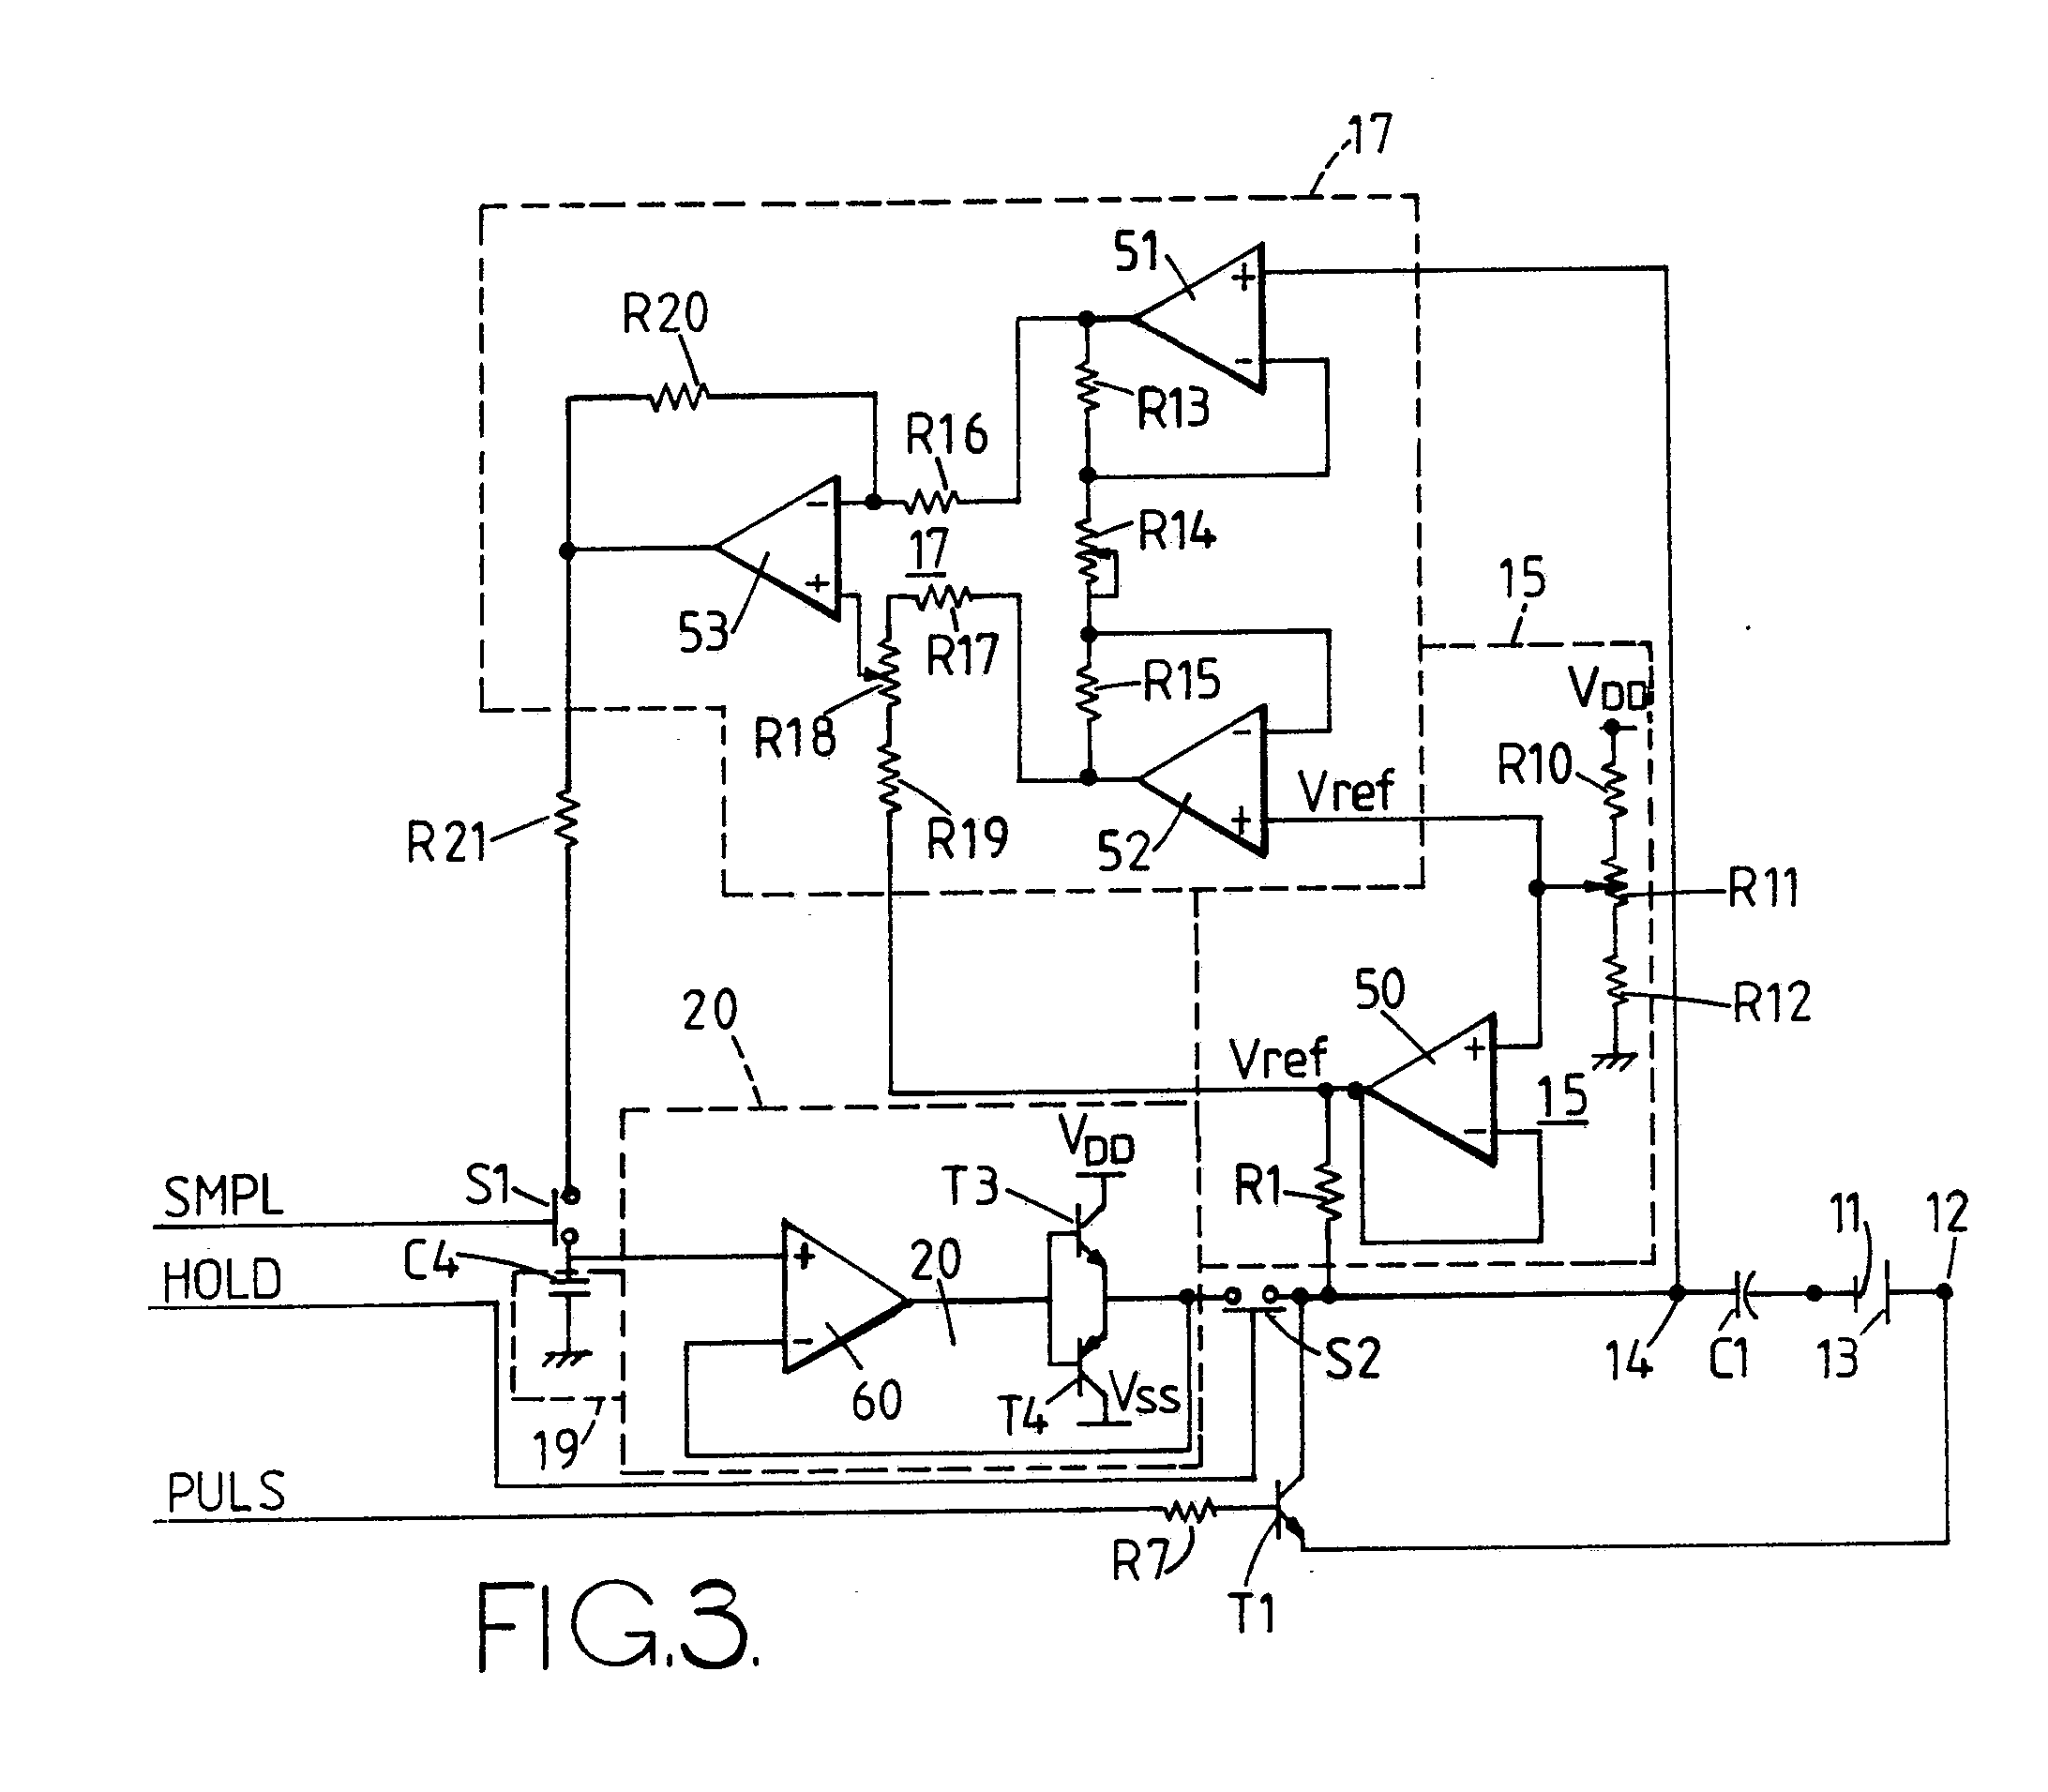
\includegraphics[width=9.9cm]{./bilder/PacemakerCircuit.png}
\end{textblock*}

\vissteduatt{Visste du att .... något mer om kth medtech eller BME? ELLER visste du att Pacemakern är en Lundauppfinning?}


\newpage


\subsection*{Mer jul} 
\index[alfa]{Mer jul}
\index[anfa]{Mer jul} 
\songinfo{Av: Falk Adolphson
}

\begin{parse lines}[\noindent]{#1\\}
    Jag är en lugn person med takt och ton
    måttfull och balanserad
    Jag är tyst och still och det ska mycket till 
    innan jag blir exalterad
    Men jag har en last som håller mig fast 
    i ett järngrepp varje vinter
    När året är slut och snön ligger djup 
    och slädarnas medar slinter

    Jag vill ha mer jul
    Ge mig mer jul
    Jag vill ha mer jul
    Ge mig mer jul
    Tusen stjärnor som tindrar,
    glitter så långt jag ser
    Av juleljus som glimmar,
    vill jag ha mer


\end{parse lines}

\newpage

\begin{parse lines}[\noindent]{#1\\}
    En show glöms bort om den bara visar opp 
    effekter som man knappast anar
    Så ge mig trettio grader kallt, tomtar överallt 
    och en skog av gröna granar
    Jag vill ha snötyngda hus, tusentals ljus, 
    kulörta kulor i drivor
    Bjällerklang som ackompanjemang 
    på alla julens skivor

    Jag vill ha mer jul…

    Ge mig en svårknäckt nöt, sötare gröt, 
    djupare dopp i grytan
    Glittrigare glim och grötigare rim 
    och mer Arne Weise i rutan
    Jag vill ha rymligare säck, segare knäck, 
    fetare fläsk från grisen
    Krimsigare krams, längre långdans 
    och raskare räv på isen

    Jag vill ha mer jul…

    Jag vill ha mer, mer
    Ge mig mer, mer
    Jag vill ha mer, mer
    Ge mig mer, mer

\end{parse lines}

\vissteduatt{Visste du att Mer Jul spelas årligen i Edekvata oavbrutet från och \\med Glöggillet fram till Julgillet är hållet?}

\newpage

\subsection*{Jag är liten nolla} 
\index[alfa]{Jag är liten nolla}
\index[anfa]{Jag är liten nolla}
\songinfo{Mel: Jag är fattig bonddräng\\
Text: JO Sivtoft, E94}

\begin{parse lines}[\noindent]{#1\\}
    Jag, en liten nolla, på Elektro jag går
    Dagar går och kommer, medan jag pluggar på
    Labbar, löddar, räknar, programmerar och lär, 
    Går på föreläsning, inför tentan jag svär

    Jag en fattig nolla, pasta lever jag på
    Och när fredan kommer till Edekvata jag gå
    Sen, när jag blitt livad, vill jag dansa, umgås
    Vila hos en flicka, vill jag också förstås

    Sen så kommer helgen, och då vill CSN
    Att jag pluggar satan, men då festar jag än
    40 timmars vecka, gäller inte för oss
    För oss teknologer, e de dubbelt förstås

    Så går hela veckan, varje läsperiod
    Åren går och kommer, men jag är vid gott mod
    Jag tar mina tentor, samlar på mig poäng, 
    Jag tar min examen, sen så blir jag utslängd

    Nu så väntar livet, som civilingenjör
    Nu så ska jag skörda, tjäna pengar som smör
    Men man jobbar sliter, si så där 40 år
    Till barn, familj o staten, alla pengarna går

    Så när dagen kommer, invid himmelens port, 
    Lite rädd och lessen, för de synder jag gjort
    Inte skattefuska, köra fort, supa loss
    Herren Gud i himlen, är väl missnöjd förstas

    Jag, vid pärleporten, blir nu eftertänksam
    De allra bästa åren, alltför snabbt de försvann
    Hade allt för bråttom, bort från de som var bäst
    Åren på Elektro, saknar jag allra mest

    Men då säger Herren: (civil) ingenjören, kom hit! 
    Jag har sett din strävan, och ditt eviga slit
    Därför, ingenjören, är du välkommen här
    Himmelens Elektro till du antagen är

    Jag som liten ängel, står så still inför Gud, 
    och sen klär han på mej en Elektrovit skrud
    Nu du, säger Herren, börjar vi om igen 
    Nu du, liten nolla, nu har du kommit hem

    Till dig liten nolla, sensmoralen den är
    Ha ej allt för bråttom, under tiden du lär
    Tids nog får du jobba, resten utav ditt liv
    Därför ta till vara, på studentlivets tid
\end{parse lines}

\vissteduatt{Visste du att... sjunges gärna på nollegasque(???)}


\newpage

\subsection*{Hacke Hackspett} 
\index[alfa]{Hacke Hackspett}
\index[anfa]{Hacke Hackspett}
\songinfo{Mel: Woody Woodpecker (Georg F. Tibbles, Ramey Idriss)\\
Text: Povel Ramel \& Georg Eliasson
}

\begin{parse lines}[\noindent]{#1\\}
     %\textit{Mitt namn är Hacke Hackspett, resande i Schweizerostar!}
    Hahahahaha! Hahahahaha! Hör på hackspettens melodi
    Hahahahaha! Hahahahaha! Med sin hackande harmoni!
    
    Han hackar sig fram
    ifrån stam till stam
    och bygger upp sitt höga C
    När du märker hans skratt,
    så ta på dig din hatt
    ty han är på jakt efter tre
    
    ||: Hahahahaha! Hahahahaha! 
    Har du hört en så’n retfull trall,
    Hahahahaha! Hahahahaha! 
    När du traskar bland gran och tall
    
    Om hans skönsång nu ej
    gör nå't intryck på dig,
    alla hackspettars hjärtan slår
    
    Hahahahaha! Hahahahaha! Varje gång det är sol och vår :||
\end{parse lines}

\vissteduatt{Visste du att Povel Ramel och hans glättiga gröngölingar spelade in\\
 låten på 78-varvare 23 september 1948?}


\newpage


% \input{kapitel/03-andra_sektioner.tex}

% \input{kapitel/04-klassiska_visor.tex}

% \input{kapitel/05-skånska_visor.tex}

% \begin{center}
    \vspace*{1.5cm}
    {\fontsize{20}{20}\textbf{Teknologvisor}}\\
    \vspace{0.7cm}
    {\fontsize{12}{12}\textit{Om teknologen själv får välja}}
\end{center}
\addtocwithheader{Teknologvisor}  % Add entry to TOC and set header\noBackground
\noBackground

\newpage
\resetBackground


\subsection*{Porthos visa} 
\index[alfa]{Porthos visa}
\index[anfa]{Jag vill börja gasqua!}
\songinfo{Mel: You can't get a man with a gun \\(ur Annie get your gun)\\Text: T Andrén}
\colorbox{yellow}{Vi måste bestämma hur texten ska vara. Samma som i förra boken \\eller ska vi följa vad vi hittar i andra böcker eller online?}

\begin{parse lines}[\noindent]{#1\\}
    Jag vill börja gasqua!
    Var fan är min flaska?
    Vem i helvete stal min butelj?
    Skall mej törsten betvinga?
    En TT börja svinga?
    Nej för fan bara blunda och svälj!
    Vilken smörja!
    Får jag spörja?
    Vem för fan tror att jag är en älg?
    Till England vi rider,
    och sedan vad det lider,
    träffar vi välan på någon PUB
    Och där skall vi festa!
    Blott dricka utav det bästa
    utav Whiskey och Portvin
    Jag tänker gå hårt in
    för att prova på rubb och stubb
    Rubb och stubb…
\end{parse lines}

\vissteduatt{Visste du att om den sista "stubb" sjunges så måste låten upprepas...}

% \newpage


\subsection*{En komplex värld} 
\index[alfa]{En komplex värld}
\index[anfa]{Alla jävla bevis}
\songinfo{Mel: En helt ny värld (ur Aladdin)\\
Text: Ellinor Persson F07 och Andreas Tågerud F06
}

\begin{parse lines}[\noindent]{#1\\}
    Alla jävla bevis
    inses lätt som en övning.
    Javakursen en prövning
    för min bristande logik.

    Ska man komma ihåg
    alla formler i huvet?
    Formelsamlingen, du vet,
    säger inget om det här!

    En komplex värld
    Vad fan betyder bijektiv?
    Ingenting stämmer här, där allt jag lär,
    blir glömt snart efter tentan.
    Hur ska det gå?
    Och det är bara vecka två...
    Känner en underton av aggression
    mot allt Sven Spanne skrivit i sin bok

    (Jag kan transponera den...)
\end{parse lines}

\newpage

\begin{parse lines}[\noindent]{#1\\}
    Jag kan lära dig C
    Matematiska under
    Oförglömliga stunder
    när vi tentar mekanik

    Det ska nog gå!
    Det sa din mamma med igår
    All tid tillvaratas, jag är i fas,
    och bor i mattehuset.
    Nu är jag lärd!
    Till denna svåra ekvation
    jag på frekvenssidan en lösning fann,
    den låg där i en helt ny värld: Laplace!
\end{parse lines}

\subsection*{Enhetsvisan / SI - Système International d'Unités} 
\index[alfa]{Enhetsvisan / SI - Système International d'Unités}
\index[anfa]{1, 2, 75, 6, 7}
\songinfo{Mel: Studentsången}

\begin{parse lines}[\noindent]{#1\\}
    W kg m Wb s
    Ω m T A rad
    cd Sv N s
    Ω A m lx dB
    °C W/m²
    J/kg H V C
    kg/m3 mol
    m/s²
    m/s²
    F !
\end{parse lines}

\vissteduatt{Visste du att SI-låttexten finns i TeFyma?}

\newpage

\subsection*{Man ska ha matlab} 
\index[alfa]{Man ska ha matlab}
\index[anfa]{Man ska ha matlab}
\songinfo{Mel: Man ska ha husvagn}

\begin{parse lines}[\noindent]{#1\\}
    Jag har prövat nästan allt som finns att pröva på
    Beta, kulram, räknesticka, tärning eller så
    Jag har kalkylerat på de konstigaste sätt
    och nu så har jag kommit på hur man ska räkna rätt

    Man ska ha MATLAB - då är kalkylen redan klar
    Man ska ha MATLAB - det har jag sett att andra har
    Man ska ha MATLAB - det är min livsfilosofi
    Man ska ha MATLAB - för då blir man fri

    I många år så var jag inte alls så särskilt lärd
    Jag visste ej vad som vänta' mig i denna stora värld
    Men sen kom jag till LTH, och ända sedan dess
    så har jag funnit livets stora lyxdelikatess

    Man ska ha MATLAB - så man slipper tänka alls
    Man ska ha MATLAB - ja, då går allting som en vals
    Man ska ha MATLAB - det bygger på nån slags logik
    Man ska ha MATLAB - för då blir man rik

    5 minuter mekanik och 5 minuter statfys
    5 minuter plottande och 5 minuter analys
    5 minuter fråga phadder, 5 minuter stopp
    5 minuter tänka själv och sen så ger man opp
\end{parse lines}

\vissteduatt{Vad kom först MATLAB eller Maple?}

\newpage

\begin{parse lines}[\noindent]{#1\\}
    Man ska ha MATLAB - och datasalens friska luft
    Man ska ha MATLAB - det tycker tjejerna är tufft
    Man ska ha MATLAB - när ryssen kommer med sitt MIG
    Man ska ha MATLAB - då vinner man i krig!
\end{parse lines}

\vissteduatt{visste du att}

\newpage

\subsection*{Teknologvisa} 
\index[alfa]{Teknologvisa}
\index[anfa]{Jag är teknolog och helt OK}
\songinfo{Mel: The Lumberjack Song (Monty Python)\\ Sångarstriden 1982\\ Kursivt sjunges av sångförman}

\noindent\textit{Jag är teknolog och helt OK\\
Jag jobbar hårt och jag roar mig}\\\\
\noindent Han är teknolog och helt OK\\
Han jobbar hårt och han roar sig\\\\
\noindent\textit{Teknik är ball\\
Jag kan Pascal\\
Till Lophtet vill jag gå\\
Där träffas alla vänner\\
som är från LTH}\\\\
\noindent Teknik är ball\\
Han kan Pascal\\
Till Lophtet vill han gå\\
Där träffas alla vänner\\
som är från LTH\\\\
\noindent För han är teknolog och helt OK\\
Han jobbar hårt och han roar sig\\\\

\vissteduatt{Visste du att "Han" kan eneklt bytas ut mot "Hon" eller "Hen"!}

\newpage

\noindent\textit{Min mattebok \\
den gör mig klok\\
Jag läser kärnfysik\\
Jag går på föreläsning\\
och älskar juridik}\\\\
\noindent Hans mattebok\\
den gör han klok\\
Han läser kärnfysik\\
Han går på föreläsning\\
och älskar juridik???\\\\
\noindent Men han är teknolog och helt OK\\
Han jobbar hårt och han roar sig\\\\
\noindent\textit{Som ekonom jag blir fantom\\
Konkurser gör mig säll\\
Till flickor blankt jag nekar\\
Jag älskar en tabell}\\\\
\noindent Som ekonom han blir fantom???\\
konkurser...\\
Nää, BUU!!\\\\
\noindent Men han är teknolog och helt OK\\
Han jobbar hårt och han roar sig\\


\newpage

\subsection*{Flerdimensionell ångest} 
\index[alfa]{Flerdimensionell ångest}
\index[anfa]{Flerdimensionell ångest}
\songinfo{Mel: Härjarevisan\\
Text: Daniel Milve F11}

\begin{parse lines}[\noindent]{#1\\}
    Jag har aldrig sett mig själv som välkalkylerad
    Riktningsderivata gör min hjärna punkterad
    Man borde börjat lyssna redan
    Typ när nollningen tog stopp
    Än har jag ingen aning om vad Green’s formel säger
    Dock vet jag klart och tydligt vad de dryga förtäljer:
    Skillnaden mellan kurs och fest är 
    Kurser kan man göra om!

    Men så nu ska vi ut och tenta
    Statens små bidrag hämta
    Differentialer, integral och vektoranalys (i planet!)
    Fem timmar med hårda tag och
    Nu änteligen lär jag
    Kunna dra nån nytta av vad Månsson sade vecka två!
\end{parse lines}

\vissteduatt{Visste du att...}


\newpage


\subsection*{O, hemska labb} 
\index[alfa]{O, hemska labb}
\index[anfa]{O, hemska labb}
\songinfo{Mel: O, helga natt}

\colorbox{orange}{OSÄKER PÅ DENNA}

\begin{parse lines}[\noindent]{#1\\}
    O, hemska labb, o grymma kval imorgon
    Här sitter jag och förstår ingenting
    Hela mitt inre är fyllt utav ett motstånd
    emot eländig elektrisk mätteknik
    Jag skulle nog behöva lite ledning,
    här räcker inte min kapacitans
    Kondensatorer och felvända dioder
    O, hemska labb nu vill jag koppla af
    O, hemska labb ty detta blir min graf

    O, hemska labb, o grymma kval imorgon
    Här sitter jag och förstår ingenting
    Hela programmet är fyllt utav funktioner
    som innehåller en himla massa fel
    Pekare som inte har nån riktning,
    oändliga loopar, oj vad jag blir sträng!
    Åh, kompilera, hur ska det här fungera?
    O, hemska labb, nu vill jag logga ut
    O, hemska labb, ty detta blir mitt slut
\end{parse lines}

\vissteduatt{Visste du att...}


\newpage


\subsection*{Tenta efter jul} 
\index[alfa]{Tenta efter jul}
\index[anfa]{Tenta efter jul}
\songinfo{Mel: Mössens julafton\\
Skriva om att D-sektionen vinnande bordvisa (SåS enligt sångarkiv)}

\colorbox{yellow}{OSÄKER PÅ DENNA}

\begin{parse lines}[\noindent]{#1\\}
    När julen börjar närmas
    och man vill koppla av
    Så kommer tentaplugget
    här och ställer sina krav

    Jag börjar kompromissa
    gör julrimmen i C
    Försöker strukturera
    pluggar fram till klockan tre

    Programmering lin-jär algebra
    Endim å reglerteknik är ingenting att ha
    Tenta efter nyår är ju trist
    Men skippar man för många ja då blir man alkolist

    Skål! 
\end{parse lines}

\vissteduatt{Visste du att...}


\newpage




% \input{kapitel/07-ölvisor.tex}

% \begin{center}
    \vspace*{1.5cm}
    {\fontsize{20}{20}\textbf{Vinvisor}}\\
    \vspace{0.7cm}
    {\fontsize{12}{12}\textit{Om den nytvättade vita skjortan själv får välja}}
\end{center}
\addtocwithheader{Vinvisor}  % Add entry to TOC and set header\noBackground
\noBackground

\newpage
\resetBackground

\subsection*{\colorbox{red}{Tar bort: Lovsången till kvinnan}} 
% \index[alfa]{Öl, öl, öl i glas}
% \index[anfa]{Öl, öl, öl i glas}
% \songinfo{Mel: Row your boat}

\begin{parse lines}[\noindent]{#1\\}
    tas bort
\end{parse lines}

\vissteduatt{Visste du att...}

\newpage

\subsection*{Feta fransyskor} 
\index[alfa]{Feta fransyskor}
\index[anfa]{Feta fransyskor}
\songinfo{Mel: Militärmarsch av Schubert\\
K-sektionen Sångarstriden 1985}

\begin{parse lines}[\noindent]{#1\\}
    Feta fransyskor som svettas om fötterna,
    de trampar druvor
    som sedan ska jäsas till vin
    Transpirationen viktig é,
    ty den ge'
    fin bouquet
    Vårtor och svampar följer me'
    men vad gör väl de'?

    För vi vill ha vin,
    vill ha vin,
    vill ha mera vin,
    även om följderna blir
    att vi må lida pin
    Flaskan och glaset gått i sin
    Hit med vin, mera vin!
    Tror ni att vi är fyllesvin?
    {\Large Ja!} (Fast större!)
\end{parse lines}

\vissteduatt{Visste du att...}


\newpage


\subsection*{Lyft ditt välförsedda glas} 
\index[alfa]{Lyft ditt välförsedda glas}
\index[anfa]{Lyft ditt välförsedda glas}
\songinfo{Mel: Ding dong merrily on high}

\begin{parse lines}[\noindent]{#1\\}
    Lyft ditt välförsedda glas
    Det är en härlig börda
    Nu har grabbarna kalas
    Ve segern snart skall skörda
    //: Ding dingedingeding dingedingeding
    dingedingeding dong dong
    Imorgon är det lördag ://

    Sätt nu glaset till din mun
    Se döden på dig väntar
    Nu har grabbarna kalas
    Hör liemannen flämtar
    //: Ding dingedingeding dingedingeding
    dingedingeding dong dong
    Begravningsklockor klämtar ://
\end{parse lines}

\vissteduatt{Visste du att...}


\newpage


\subsection*{Bordeaux, bordeaux} 
\index[alfa]{Bordeaux, bordeaux}
\index[anfa]{Jag minns än idag hur min fader}
\songinfo{Mel: I sommarens soliga dagar}

\begin{parse lines}[\noindent]{#1\\}
    Jag minns än idag hur min fader
    kom hem ifrån staden så glader
    och rada' upp flaskor i rader
    och sade nöjd som så:
    "Bordeaux, Bordeaux!"

    Han drack ett glas, kom i extas,
    och sedan blev det stort kalas
    Och vi små glin, ja vi drack vin
    som första klassens fyllesvin
    Och vi dansade runt där på borden
    och skrek så vi blev blå:
    "Bordeaux, Bordeaux!"
\end{parse lines}

\vissteduatt{Visste du att...}


\newpage


\subsection*{Vinbröder} 
\index[alfa]{Vinbröder}
\index[anfa]{Två bröder, Jan-Ove och Hadar}
\songinfo{Mel: I sommarens soliga dagar}

\begin{parse lines}[\noindent]{#1\\}
    Två bröder, Jan-Ove och Hadar,
    de plockade fram sina spadar,
    och grävde en grop bakom huset.
    De hade en idé:
    Vaddå, vaddå?
    Jo, priset på 
    Kir och Bordeaux,
    är högt men om man gjorde så,
    att man i gropen lade ner,
    två kilo jäst och en back MER,
    så skulle det nog vara möjligt
    att producera vin i detta hål! Skål!
\end{parse lines}

\vissteduatt{Visste du att...}


\newpage


\subsection*{Karnaugh, karnaugh} 
\index[alfa]{Karnaugh, karnaugh}
\index[anfa]{Karnaugh, karnaugh}
\songinfo{Mel: I sommarens soliga dagar}

\begin{parse lines}[\noindent]{#1\\}
    Jag minns än i dag hur min fader
    kom hem i från labbet så glader
    och rada' upp bitar i rader
    och sade glad som så:
    Karnaugh, Karnaugh!

    Å ett å noll \& noll å ett 
    å booleska uttryck det är fett!
    Med ett å noll \& noll å ett,
    ska du nu se att det blir rätt,
    Men vi felsökte våra signaler,
    och det blev fel ändå
    Karnaugh, Karnaugh!
\end{parse lines}

\vissteduatt{Visste du att...}


\newpage


\subsection*{I sommarens soliga dagar} 
\index[alfa]{I sommarens soliga dagar}
\index[anfa]{I sommarens soliga dagar}
\songinfo{Mel: I sommarens soliga dagar\\
Text: Anders Nilsson $\pi$03 och Björn Carlin $\pi$02}

\begin{parse lines}[\noindent]{#1\\}
    I sommarens soliga dagar
    Kall rå fisk till alla vi lagar
    Och sätter oss ute i hagar
    Där maten härsken står
    Bakteriehärd av solen närd
    Den höjer högt sitt blanka svärd
    Men mot dess hot vi funnit bot 
    Vi sätter spritens krafter mot
    För spriten kan döda det mesta
    Vi hälsan återfår, Gutår! Gutår!
\end{parse lines}

\vissteduatt{Visste du att...}


\newpage


\subsection*{Kosmetisk visa} 
\index[alfa]{Kosmetisk visa}
\index[anfa]{Du behöver inte ha nåt läppstift alls}
\songinfo{Mel: She’ll be Coming ‘Round the Mountain\\
Lundakarnevalen 2002}

\begin{parse lines}[\noindent]{#1\\}
    Du behöver inte ha nåt läppstift alls,
    du behöver inte ha nåt läppstift alls,
    för när vinet börjar flöda,
    färgas läpparna ju röda,
    liksom tungan, hakan, skjortan och din hals!
\end{parse lines}

\vissteduatt{Visste du att...}


\newpage


\subsection*{Magnumflaskan Åkesson} 
\index[alfa]{Magnumflaskan Åkesson}
\index[anfa]{Magnumflaskan Åkesson}
\songinfo{Mel: Teddybjörnen Fredriksson\\
Lundakarnevalen 2010}

\begin{parse lines}[\noindent]{#1\\}
    För längesen, när jag fyllde 15 år
    fick jag en flaska av min mor
    Hon sa "Mitt barn, dela den med vännerna
    För den är faktiskt ganska stor."

    Magnumflaskan Åkesson,
    du var så stor och tung
    Jag gick runt med dig i hand,
    och i Dalby var jag kung

    Magnumflaskan Åkesson,
    din kork försvann i skyn
    Men jag drack dig bara själv
    Och kräktes i hela byn
\end{parse lines}

\vissteduatt{Visste du att...}


\newpage


\subsection*{\colorbox{orange}{Korkskruvens visa}} 
% \index[alfa]{Magnumflaskan Åkesson}
% \index[anfa]{Magnumflaskan Åkesson}
\songinfo{Mel: Nu har vi ljus}

\begin{parse lines}[\noindent]{#1\\}
    TA BORT???

    Nu har vi rus här i vårt hus
    Korken är borta hopptralalala
    Doften är ljuv, jag är en skruv,
    jag är en skruv.

    Jag kan inte öppna bag-in-boxen,
    jag kan inte öppna bag-in-boxen

    Lalalala lalalala lalalalala lala
\end{parse lines}

\vissteduatt{Visste du att...}


\newpage


\subsection*{Dance macabre} 
\index[alfa]{Dance macabre}
\index[anfa]{runt våran stuga, små djävlar sluga}
\songinfo{Mel: Vårvindar friska}

\begin{parse lines}[\noindent]{#1\\}
    Runt våran stuga, små djävlar sluga
    tassa så tyst med bockfot och svans
    Varulvar yla, isande kyla
    sveper i dimman, fantygets dans
    Bäva, o broder, lyssna och hör
    vrålen från gast, som osalig dör
    Satan han skrattar,
    flaskan han fattar,
    super tills dagen gryr.

    Gastar och spöken
    skymta i köken,
    dödingar släpa ruttnande lik
    Benrangel skramla,
    spökhänder famla,
    kväva din strupes rosslande skrik
    Helvetes alla fasor släpps loss
    Fan rider här med hela sin tross
    Göm dig i stugan,
    du har fått flugan
    Dille det blir din lott

\end{parse lines}

\vissteduatt{Visste du att man viskar hela låten fram till \\ "Helvetets alla fasor..." då tar man i för Kung och fosterland?}


\newpage




%\begin{center}
    \vspace*{1.5cm}
    {\fontsize{20}{20}\textbf{Snapsvisor}}\\
    \vspace{0.7cm}
    {\fontsize{12}{12}\textit{Om helan själv får välja}}
\end{center}
\addtocwithheader{Snapsvisor}  % Add entry to TOC and set header\noBackground
\noBackground

\newpage
\resetBackground

\begin{textblock*}{3cm}(0.0cm,0.2cm) % {width}(x, y)
    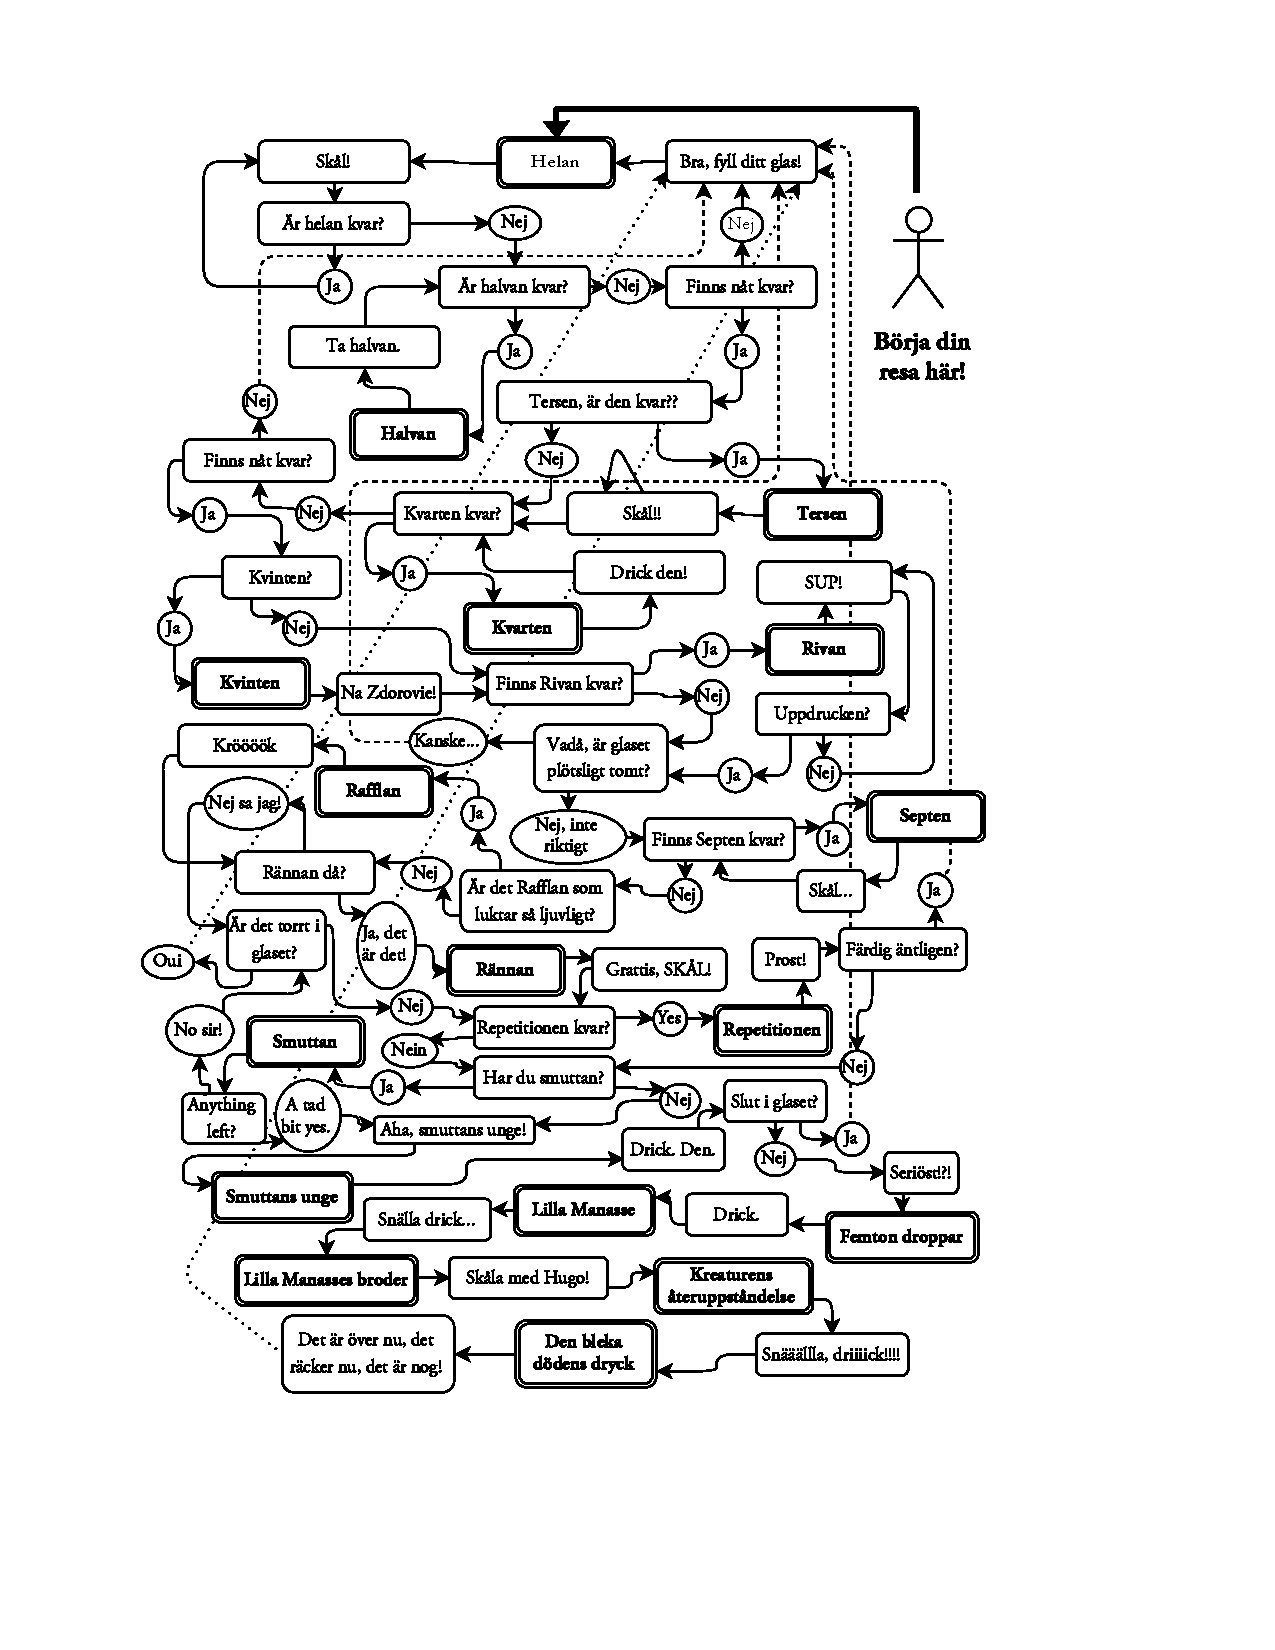
\includegraphics[width=12cm]{./bilder/SupSchema_FINAL_2.pdf}
\end{textblock*}

osynlig text

\vissteduatt{Har du kommit fram till "Den bleka dödens dryck" har du varit \\mycket sparsam. Bra jobbat!}

\newpage

\subsection*{Törsten rasar} 
\index[alfa]{Törsten rasar}
\index[anfa]{Törsten rasar uti våra strupar}
\songinfo{Mel: Längtan till landet}

\begin{parse lines}[\noindent]{#1\\}
    Törsten rasar uti våra strupar,
    tungan hänger torr och styv och stel
    Men snart vankas stora, kalla supar,
    var och en får sin beskärda del
    Snapsen kommer, den vi vilja tömma,
    denna nektar lik Olympens saft,
    kommer oss att våra sorger glömma
    Snapsen skänker hälsa, liv och kraft

    Fordom odlade man vindruvsranka,
    av vars frukt man gjorde ädelt vin
    Nu man pressar saften ur en planka,
    doftande av äkta terpentin
    Höj din bägare, O, Broder, yster,
    och låt svenska skogen glida kall,
    ner för strupen och om sen det dig lyster,
    låt oss supa opp en liten tall
\end{parse lines}

\vissteduatt{Visste du att funktionärsposten macapär infördes efter att sektionen\\köpt sin första Mac?}

\newpage

\begin{parse lines}[\noindent]{#1\\}
    Helan tänder helig eld i själen,
    halvan rosar livet som en sky
    Tersen känns från hjässan ner i hälen,
    kvarten gör oss till en mänska ny
    Låt oss skåla med varann, go' vänner,
    skål för våran levnads glada lopp,
    törstens eld på nytt i strupen bränner
    Leve livet! Skål och botten opp!

\end{parse lines}

\subsection*{Helan går} 
\index[alfa]{Helan går}
\index[anfa]{Helan går}
\songinfo{Kursivt sjunges av sångförman}

\begingroup
\itshape
\noindent Det satt en liten fågel på en gren\\
\noindent och sjöng i furuskogen\\
\noindent Han hade sjungit hela dagen lång,\\
\noindent men dock ej sjungit nog än\\
\noindent Men vad sjöng den lilla fågeln då?\\
\noindent Jo! Han sjöng:\\
\endgroup

\begin{parse lines}[\noindent]{#1\\}
    Helan går,
    sjung hopp faderallan lallan lej,
    Helan går,
    sjung hopp faderallan lej.
    Och den som inte helan tar,
    han heller inte halvan får
    Helan går,
    sjung hopp faderallan lej
\end{parse lines}

\newpage

\subsection*{Samling vid pumpen} 
\index[alfa]{Samling vid pumpen}
\index[anfa]{Samling vid pumpen}
\songinfo{Mel: Hujedamej sån’t barn han var}

\begin{parse lines}[\noindent]{#1\\}
    Samling nu vid pumpen 
    alla ni som dricker vatten 
    Vi som dricker brännvin 
    vi höjer våra glas 
    Vatten ska man ha 
    när man ska vattna i rabatten 
    Brännvin ska man ha 
    när man e på kalas!

\end{parse lines}


\subsection*{Inre dialog} 
\index[alfa]{Inre dialog}
\index[anfa]{Jag vill inte ha}
\songinfo{Mel: An der Schönen Blauen Donau\\
Kursivt sjunges av sångförman}

\textit{Jag vill inte ha} \hfill En nubbe till! \hspace*{15pt} \\
\textit{Jag  mår inte bra} \hfill En nubbe till! \hspace*{15pt} \\
\textit{Om ni ger mig mer} \hfill En nubbe till! \hspace*{15pt} \\
\textit{ser jag er som fler} \hfill En nubbe till! \hspace*{15pt} \\
\textit{Min mage är sjuk} \hfill En nubbe till! \hspace*{15pt} \\
\textit{Min hjärna är mjuk} \hfill En nubbe till! \hspace*{15pt} \\
\\
\textit{Jag kan inte tääänkaaa så braaa}\\
\textit{så jag får väl nubben ta} \hfill HURRA! \hspace*{37pt} 

\vissteduatt{Visste du att rummet Pump heter Pump eftersom fontänens pump\\tidigare stod i det rummet?}

\newpage


\subsection*{Tänk om jag hade lilla nubben} 
\index[alfa]{Tänk om jag hade lilla nubben}
\index[anfa]{Tänk om jag hade lilla nubben}
\songinfo{Mel: Hej, tomtegubbar}

\begin{parse lines}[\noindent]{#1\\}
    Tänk om jag hade lilla nubben
    uppå ett snöre i halsen
    Tänk om jag hade lilla nubben
    uppå ett snöre i halsen
    Jag skulle dra den upp och ner
    så att det kändes som många fler
    Tänk om jag hade lilla nubben
    uppå ett snöre i halsen

\end{parse lines}

\subsection*{Livet är härligt} 
\index[alfa]{Livet är härligt}
\index[anfa]{Livet är härligt}
\songinfo{Mel: Röda kavalleriet \\ Ur Chalmersspexet Katarina II 1959}

\begin{parse lines}[\noindent]{#1\\}
    Livet är härligt
    Tavarisjtj, vårt liv är härligt
    Vi alla våra små bekymmer glömmer
    när vi har fått en tår på tanden, SKÅL!

    Tag dig en vodka
    Tavarisjtj, en liten vodka
    Glasen i botten vi tillsammans tömmer;
    det kommer mera efter hand

    En SKÅL!
\end{parse lines}

\vissteduatt{Visste du att fler skånska snapsvisor finns på sida 74?}
\newpage


\begin{textblock*}{3cm}(5.3cm,9.5cm) % {width}(x, y)
    
\includegraphics[width=4.5cm]{./bilder/GalenVetenskapsmanTransparent.png}
\end{textblock*}

\subsection*{Det naturliga urvalet} 
\index[alfa]{Det naturliga urvalet}
\index[anfa]{Darwin studerade liv och natur}
\songinfo{Mel: Mors lilla Olle\\
Text: Rolf Malmström}

\begin{parse lines}[\noindent]{#1\\}
    När Darwin studerade liv i natur
    Så fann han att först dör de svagaste djur
    De sämsta bland hjärnceller dör också först
    Så öka din IQ och minska din törst

\end{parse lines}

\subsection*{Lillebror och jag} 
\index[alfa]{Lillebror och jag}
\index[anfa]{Tycker du att snapsen är för stor}
\songinfo{Mel: Måltidssången (refrängen)\\
Lundakarnevalen 1998}

\begin{parse lines}[\noindent]{#1\\}
    Tycker du att snapsen är för stor
    kan du ge en slatt till lillebror
    Både en, både två, både tre, både fem
    och sen blir det fosterhem!

\end{parse lines}


\subsection*{Talteori} 
\index[alfa]{Talteori}
\index[anfa]{1, 2, 75, 6, 7}
\songinfo{Mel: Ritch, ratch}

\begin{parse lines}[\noindent]{#1\\}
    1, 2, 75, 6, 7, 75, 6, 7, 75, 6, 7,
    1, 2, 75, 6, 7, 75, 6, 7, 73,
    107, 103, 102,
    107, 6, 19, 27,
    17, 18, 16, 15,
    13, 19, 14, 17,
    19 16 18 11 
    8 47!
\end{parse lines}
\enlargethispage{1cm}
\newpage

\subsection*{Vikingen} 
\index[alfa]{Vikingen}
\index[anfa]{En viking vill ha livets vann}
\songinfo{Mel: When Johnny comes marching home\\
Text: Olof Ekdahl\\
E-sektionen Sångarstriden 1981}

\begin{parse lines}[\noindent]{#1\\}
    
    En viking vill ha livets vann,
    hurra, hurra!
    Den hastigt i mitt svalg försvann,
    hurra, hurra!
    Till kalv, till oxe, till fisk, till fläsk,
    när kärringen bara dricker läsk,
    då vill alla sanna vikingar ha en bäsk

    När vi druckit bäsken slut,
    tragik, tragik!
    Då bäres varje viking ut,
    som lik sig lik
    Och sen, om vi vaknar, vi sjunger en bit,
    sen korkar vi upp Skånes Akvavit
    ||: Skål för alla vikingar som kom hit!:|| 
\end{parse lines}

\vissteduatt{Visste du att Vikingen skrevs av en E:are? Han heter Olof,\\kallades Öloph, och var sektionens första krögare.}

\newpage

\begin{textblock*}{3cm}(6.1cm,8.5cm) % {width}(x, y)
    
\includegraphics[width=4cm]{./bilder/majas-bilder/devil.png}
\end{textblock*}

\subsection*{Imbelupet} 
\index[alfa]{Imbelupet}
\index[anfa]{Imbelutpet glaset står på bräcklig fot}
\songinfo{Mel: Kors på Idas grav}

\begin{parse lines}[\noindent]{#1\\}
    Imbelupet glaset står på bräcklig fot,
    kalla pilsnerpavor luta sig därmot
    men därnere, miserere,
    uti magens dunkla djup,
    sitter djävulen och väntar på en sup

    uti magens välvda valv, 
    vankar djävulen och ropar på en halv

    uti magen härs och tvärs,
    kilar djävulen och skriker på en ters

    uti magen djup så svart,
    löper djävulen och skränar på en kvart

    uti magens labyrint,
    irrar djävulen och tjoar på en kvint

    uti magens slingerväxt,
    springer djävulen och skriar på en sext

    uti magen heluppknäppt
    rusar djävulen och vrålar på en sept!

    uti magen an och av
    vankar djävulen och väser på oktav
\end{parse lines}

\vissteduatt{Visste du att det finns ett svärd på sektionen? Fråga någon i 
\\KM om Sexmästarsvärdet!}
\newpage

\subsection*{Vi skålar för våra vänner} 
\index[alfa]{Vi skålar för våra vänner}
\index[anfa]{Vi skålar för våra vänner}
\songinfo{Mel: Flickan går i ringen}

\begin{parse lines}[\noindent]{#1\\}
    Vi skålar för våra vänner
    och dom som vi känner
    och dom som vi inte känner
    dom skiter vi i!

    Vi skiter i våra vänner
    och dom som vi känner
    och dom som vi inte känner
    dom skålar vi för!
\end{parse lines}

\subsection*{Den som spar den har} 
\index[alfa]{Den som spar den har}
\index[anfa]{Om man bara tar en smutt, smutt, smutt}
\songinfo{Mel: Nu är glada julen slut}

\begin{parse lines}[\noindent]{#1\\}
    Om man bara tar en 
    smutt, smutt, smutt,
    utav denna lilla 
    hutt, hutt, hutt
    har man ganska mycket kvar,
    men se den som spar han har, 
    inte särskilt roligt
\end{parse lines}

\vissteduatt{Visste du att det finns ett svärd på sektionen? Fråga någon i 
\\E6 om Krögarsvärdet!}

\newpage

\subsection*{Att fela är mänskligt} 
\index[alfa]{Att fela är mänskligt}
\index[anfa]{Trampa på ett smådjur}
\songinfo{Mel: Prästens lilla kråka\\
Lundakarnevalen 2010}

\begin{parse lines}[\noindent]{#1\\}
    Trampa på ett smådjur,
    slakta gulligt rådjur,
    måste göras rätt försiktigt...

    Gifta sig med släkten,
    stjäla ur kollekten,
    det är fel och det är viktigt!

    ||: Men att sjunga en snutt, och ta sig en hutt
    Det är bara rätt och riktigt! :||
\end{parse lines}

\subsection*{Vår höga skatt} 
\index[alfa]{Vår höga skatt}
\index[anfa]{Vår höga skatt, skatt, skatt}
\songinfo{Mel: En kulen natt\\
M-sektionen Sångarstriden 2003}

\begin{parse lines}[\noindent]{#1\\}
    Vår höga skatt, skatt, skatt
    Gör att jag korsar
    En bro till främmande, främmande land
    Där spriten forsar
    Och där jag handlade, handlade sprit
    Som jag sen smugglade, smugglade hit
    Så att en su-petti-petti-petti-pett
    Jag kan få ta
    I detta nu!
\end{parse lines}

\newpage

\subsection*{Häll upp en} 
\index[alfa]{Häll upp en}
\index[anfa]{Häll upp en, häll upp en}
\songinfo{Mel: Pilutta dig\\
E-sektionen Sångarstriden 2000}

\begin{parse lines}[\noindent]{#1\\}
    Häll upp en, häll upp en
    Hell, uppenbart att jag är full
    Du får en, du får en,
    du fåren dom har ull
    Så fort man börjat snapsa har,
    man dricker tills dess inget finnes kvar,
    det kanske, det kanske, det kan skena iväg

    Mitt Valhall, mitt Valhall,
    mitt val - Hallands, det gör så gott
    I magen, I magen, i magen min är flott
    Finess och stil är mitt gebit,
    jag biter aldrig av när jag får sprit,
    jag tar en, jag tar en, jag tar en jäkel till!
\end{parse lines}

\newpage


\subsection*{En gång i månan} 
\index[alfa]{En gång i månan}
\index[anfa]{En gång i månan är månen full}
\songinfo{Mel: Mors lilla Olle}

\begin{parse lines}[\noindent]{#1\\}
    En gång i månan är månen full,
    Men aldrig vi sett honom ramla omkull
    Stum av beundran hur mycket han tål,
    Höja vi glasen och dricka hans skål!

\end{parse lines}


\subsection*{Mjölkade en ko} 
\index[alfa]{Mjölkade en ko}
\index[anfa]{Jag mjölkade en ko idag}
\songinfo{Mel: Jag fångade en räv}

\begin{parse lines}[\noindent]{#1\\}
    Jag mjölkade en ko idag 
    Men när jag såg juvret 
    Då hade jag nog tagit fel 
    För gladast var nog tjuren

\end{parse lines}

\subsection*{Dricka upp} 
\index[alfa]{Dricka upp}
\index[anfa]{Visst kan man dricka långsamt}
\songinfo{Mel: Här kommer Pippi Långstrump}

\begin{parse lines}[\noindent]{#1\\}
    Visst kan man dricka långsamt,
    hälla opp eller ner eller ingen ta
    Visst kan man dricka långsamt,
    men det tänker inte jag!
\end{parse lines}

\newpage
\noBackground

\begin{textblock*}{3cm}(5.5cm,2.8cm) % {width}(x, y)
    
\includegraphics[width=4.5cm]{./bilder/snus.png}
\end{textblock*}


\subsection*{Jag har aldrig varit på snusen} 
\index[alfa]{Jag har aldrig varit på snusen}
\index[anfa]{Jag har aldrig varit på snusen}
\songinfo{Mel: O så saligt att få vandra}

\begin{parse lines}[\noindent]{#1\\}
    Jag har aldrig vatt på snusen,
    aldrig rökat en cigarr - halleluja!
    Mina dygder äro tusen,
    inga syndiga laster jag har

    Jag har aldrig sett nå't naket,
    inte ens ett litet nyfött barn
    Mina blickar går mot taket,
    därmed undgår jag frestarens garn

    ||: Halleluja - halleluja! :||

    Bachus spelar på gitarren,
    Satan spelar på sitt handklaver
    Alla djävlar dansar tango,
    säg vad kan man väl önska sig mer?

    Jo, att alla bäckar vore brännvin,
    stadsparksdammen full av bayerskt öl,
    konjak i varenda rännsten
    och punsch i varendaste pöl

    Och mera öl…
    Vomera öl…
\end{parse lines}

\vissteduatt{Visste du att de första BME-studenterna började på \\
LTH först 2011?}
\newpage
\resetBackground

\subsection*{Jag har aldrig varit på UB} 
\index[alfa]{Jag har aldrig varit på UB}
\index[anfa]{Jag har aldrig varit på UB}
\songinfo{Mel: O så saligt att få vandra\\
E-sektionen Sångarstriden 2009}

\begin{parse lines}[\noindent]{#1\\}
    Jag har aldrig varit på UB,
    aldrig pluggat på Café Athen,
    aldrig skurit upp en snubbe,
    kan ej skilja artär från ven

    Jag har aldrig börjat klockan 9,
    eller slutat 14:32
    I AF-borgen går jag vilse,
    för jag går på LTH

    Dom har aldrig var't på ön Ön,
    aldrig målat Väg och Vattens spik
    Aldrig haft det stora nöjet,
    att få somna till Böijers logik

    Dom har aldrig vunnit en Regatta,
    eller festat i en skitig overall
    Aldrig däckat bakom Lophtet,
    för dom går ej på LTH

    E kan j-omega och Ohms lag
    F och Nano fattar kvantfysik
    Eko, eko, eko, eko,
    eko, eko med akvavit

\end{parse lines}

\newpage

\begin{parse lines}[\noindent]{#1\\}

    I och M kan ragga på kemister
    Data knackar på sin kära linuxkod
    Inga här är humanister,
    för vi är alla LTH

    I och M kan ragga på kemister
    Data knarkar på sin kära linuxkod
    Mardrömmar om humanister,
    drömmer alla på LTH

\end{parse lines}


\subsection*{The BASIC song} 
\index[alfa]{The BASIC song}
\index[anfa]{LET oss nu fatta}
\songinfo{Mel: Mors lilla Olle}

\begin{parse lines}[\noindent]{#1\\}
    \textcolor{gray}{\texttt{10}} \texttt{LET} oss nu fatta i våra glas 
    \textcolor{gray}{\texttt{20}} \texttt{INPUT} en klunk utav det som där has 
    \textcolor{gray}{\texttt{30}} \texttt{IF} du fått nog \texttt{THEN} till \texttt{50} min vän 
    \textcolor{gray}{\texttt{40}} \texttt{ELSE GOTO}-baka till \texttt{10} igen 
    \textcolor{gray}{\texttt{50}} \texttt{END}

\end{parse lines}


\vissteduatt{Visste du att innan pandemin skrevs alla programmeringstentor\\
 med papper och penna?}
\newpage



\begin{textblock*}{3cm}(5.2cm,7.5 cm) % {width}(x, y)
    
\includegraphics[width=4.0cm]{./bilder/ub.png}
\end{textblock*}




\subsection*{De som är nyktra} 
\index[alfa]{De som är nyktra}
\index[anfa]{De som är nyktra}
\songinfo{Mel: Du är den ende}

\begin{parse lines}[\noindent]{#1\\}
    De som är nyktra 
    har inte så roligt,
    de har bara ansvar 
    och inte nåt 
    tjolittanlej faderulla 
    men vi som är fulla 
    vi har bara kul nästan jämt

    Det sägs att en män'ska 
    kan va' utan brännvin,
    det stämmer måhända 
    men se blott på den min
    som pryder en absolutist, 
    den e' jävligt trist
    därför så sjunger vi nu:

    De som är nyktra 
    har inte så roligt,
    de har bara ansvar 
    och inte nåt 
    tjolittanlej faderulla 
    men vi som är fulla 
    vi har bara kul nästan jämt
\end{parse lines}

\vissteduatt{Visste du att 1996 började 272 teknologer på E? De var indelade i\\8 klasser med ungefär 32 i varje.}
\newpage


\subsection*{Vi som är nyktra} 
\index[alfa]{Vi som är nyktra}
\index[anfa]{Vi som är nyktra}
\songinfo{Mel: Du är den ende}

\begin{parse lines}[\noindent]{#1\\}
    Vi som är nyktra
    vi har faktiskt roligt.
    Jo visst har vi ansvar,
    men minst lika
    tjolittanlej faderulla
    som ni som är fulla
    som tror ni har kul nästan jämt

    Men tänk då efter
    uppå dagen efter
    de dagar med fester,
    med smärtsamma rester
    utav eran hjärna,
    nog tycker ni gärna.
    Att va nykterist är nåt visst

    Vi som är nyktra,
    vi har bara roligt
    Imorrn kan vi
    återigen ha det
    tjolittanlej faderulla,
    men ni som är fulla
    aj, aj, aj, det är väl för trist
\end{parse lines}



\newpage

\subsection*{Mera brännvin} 
\index[alfa]{Mera brännvin}
\index[anfa]{Mera brännvin i glasen}
\songinfo{Mel: Internationalen}

\begin{parse lines}[\noindent]{#1\\}
    Mera brännvin i glasen,
    mera glas på vårt bord,
    mera bord på kalasen,
    mer kalas på vår jord

    Mera jordar med måne,
    mera månar i mars,
    mera marscher till Skåne,
    mera Skåne, Gud bevars, bevars, bevars!
\end{parse lines}

\subsection*{En kulen snaps} 
\index[alfa]{En kulen snaps}
\index[anfa]{En kulen snaps}
\songinfo{Mel: En kulen natt}

\begin{parse lines}[\noindent]{#1\\}
    En kulen snaps, snaps, snaps
    Den står vid faten
    Om jag nu vågade, vågade
    ta den före maten
    Men värden håller ett jäkla långt tal
    Kanske min snaps inte längre hålls sval
    Så ner i djupetetetet
    Den snapsen slank
    Menns den var kall!
\end{parse lines}

\vissteduatt{Visste du att det finns en finsk version av Mera Brännvin?\\Se Internationella visor!}

\newpage


\subsection*{Feministvikingen} 
\index[alfa]{Feministvikingen}
\index[anfa]{En viking viker tvätten själv}
\songinfo{Mel: When Johnny Comes Marching Home}

\begin{parse lines}[\noindent]{#1\\}
    En viking viker tvätten själv
    Hurra hurra!
    Ordet "viking" kommer sig därav, jaha!
    Föräldraledigheten delas exakt
    När vikingen sina barn har lagt
    Då är vikingens fru ute på jakt

    En viking vill ha livets vann
    Hurra hurra!
    Men på sig själv han lägger band,
    Jaha, vad bra!
    Mjödet prioriteras sist,
    Tvätta och städa blir aldrig trist
    För våran viking, han är feminist
\end{parse lines}

\subsection*{Änglahund} 
\index[alfa]{Änglahund}
\index[anfa]{Det står en hund}
\songinfo{Mel: Marseljäsen
\\ V-sektionen sångarstriden 1991}

\begin{parse lines}[\noindent]{#1\\}
    Det står en hund på fjärde våningen 
    och den tänker hoppa ner!
    BANZAI!
    Det var en japanesisk självmordhund 
    och den hoppar aldrig mer!
\end{parse lines}



\newpage

\subsection*{Nu dags taga sig en snaps strax} 
\index[alfa]{Nu dags taga sig en snaps strax}
\index[anfa]{Nu dags taga sig en snaps strax}
\songinfo{Mel: Can-Can}

\begin{parse lines}[\noindent]{#1\\}
    Nu dags
    taga sig en snaps strax,
    som din kropp tar opp och
    låter rinna ner
    Och ger dig smak för flera

    Ditt liv,
    blott ett tidsfördriv, du 
    kastar ner en kask och 
    lever glatt och ler,
    när fler du ser

    Med sill,
    eller vad du vill till,
    håll din strupe våt, åt
    Bacchus ge din själ,
    han vill dig bara väl

    Så skjut 
    först en kort salut ut
    nu tar sången slut, trut
    Gapa, svälj och njut!
\end{parse lines}

\vissteduatt{Visste du att E-sektionen var först på LTH att införa ett\\permanent alkoholtillstånd?}
\newpage
\noBackground

\begin{textblock*}{3cm}(6.7cm,1.0cm) % {width}(x, y)
    
\includegraphics[width=1.4cm]{./bilder/humla.png}
\end{textblock*}
\begin{textblock*}{3cm}(7.2cm,2.2cm) % {width}(x, y)
    
\includegraphics[width=3cm]{./bilder/humla_signerad.png}
\end{textblock*}
\begin{textblock*}{3cm}(6.9cm,4.9cm) % {width}(x, y)
    
\includegraphics[width=1.6cm]{./bilder/humla.png}
\end{textblock*}
\begin{textblock*}{3cm}(8.0cm,5.9cm) % {width}(x, y)
    
\includegraphics[width=2cm]{./bilder/humla.png}
\end{textblock*}
\begin{textblock*}{3cm}(6.0cm,9.0cm) % {width}(x, y)
    
\includegraphics[width=1.4cm]{./bilder/humla.png}
\end{textblock*}

\subsection*{Humlorna} 
\index[alfa]{Humlorna}
\index[anfa]{Vi äro små humlor vi bzz, bzz}
\songinfo{Mel: Här kommer Karl-Alfred boy}

\begin{parse lines}[\noindent]{#1\\}
    ||: Vi äro små humlor vi bzz, bzz :||
    Vi äro små humlor som tar oss en geting
    Vi äro små humlor vi bzz, bzz

    ||: Vi äro små fiskar vi blubb, blubb :||
    Vi äro små fiskar som tar oss en kallsup
    Vi äro små fiskar vi blubb, blubb

    ||: Vi äro små änglar vi flax, flax :||
    Vi äro små änglar som tar oss en Djävel
    Vi äro små änglar vi flax, flax
\end{parse lines}

\subsection*{Stopp en stund} 
\index[alfa]{Stopp en stund}
\index[anfa]{Stopp en stund med skratt och pratet}
\songinfo{Mel: Räven raskar över isen}

\begin{parse lines}[\noindent]{#1\\}
    Stopp en stund med skratt och pratet,
    kniv och gaffel lägg på fatet
    Seden är, att så här,
    man handskas med destilatet

    Man lyfter glaset med höger hand,
    och trycker läpparna mot dess rand
    Man dricker ur, och grinar sur,
    och väntar på resultatet
\end{parse lines}

\newpage
\resetBackground

%\begin{center}
    \vspace*{1.5cm}
    {\fontsize{20}{20}\textbf{Rekursiva visor}}\\
    \vspace{0.7cm}
    {\fontsize{12}{12}\textit{Om tålamodet själv får välja}}
\end{center}
\addtocwithheader{Rekursiva visor}  % Add entry to TOC and set header\noBackground
\noBackground

\newpage
\resetBackground

\subsection*{Min gode vän Joel} 
\index[alfa]{Min gode vän Joel}
\index[anfa]{Min gode vän Joel}
\songinfo{Mel: Trampa på gasen}

\begin{parse lines}[\noindent]{#1\\}
    Min gode vän Joel
    Han är en glad kamrat
    Han har äpplen fram och en kulvert bak
    Min gode vän Joel
    Han ser rätt lustig ut
    Man kan kalla honom Knut
    Om man vill
    Och det vill man
\end{parse lines}

\subsection*{Vår gode vän Jor-el} 
\index[alfa]{Vår gode vän Jor-el}
\index[anfa]{Vår gode vän Jor-el}
\songinfo{Lundakarnevalen 2002}

\begin{parse lines}[\noindent]{#1\\}
    Vår gode vän Jor-El
    Är far till Superman
    Super man som han blir man full som fan
    Min gode vän Jor-El
    Han dricker supersprit
    Men tål inte kryptonit
    Kastar upp i raketen
\end{parse lines}


\newpage

\subsection*{Min Gode Vän Josef} 
\index[alfa]{Min Gode Vän Josef}
\index[anfa]{Min Gode Vän Josef}
\songinfo{Lundakarnevalen 2006}

\begin{parse lines}[\noindent]{#1\\}
    Min gode vän Josef
    Han var på fyllefest
    I tequilarace - han drack allra mest
    Den helige ande
    Slog till och passa på
    Maria kunde inte gå
    På nio månader
\end{parse lines}

\subsection*{Bortom IT-Samhället} 
\index[alfa]{Bortom IT-Samhället}
\index[anfa]{Usama Bin-Ladin}
\songinfo{Lundakarnevalen 2002}

\begin{parse lines}[\noindent]{#1\\}
    Usama Bin-Ladin
    Har ingen SMS
    Ingen ICQ eller mailadress
    Usama Bin-Ladin
    Tycks ha gått upp i rök
    Man kan inte trycka "Sök"
    Om man vill
    Och det vill Bush
\end{parse lines}

\vissteduatt{Visste du att E-sektionen var den sista sektionen på LTH att skapa\\ en egen sångbok?}

\newpage

\subsection*{Jag pluggar på LU} 
\index[alfa]{Jag pluggar på LU}
\index[anfa]{Jag pluggar på LU}
%\songinfo{}
\begin{parse lines}[\noindent]{#1\\}

    Jag pluggar på LU
    Och läser gratispoäng
    När ni gör er labb
    Ligger jag i säng
    Jag pluggar på LU
    Tar inga hårda tag
    Men ändå får jag bidrag
    Från CSN
    Ja, det får jag   

\end{parse lines}

\subsection*{Jag kuggade tentan} 
\index[alfa]{Jag kuggade tentan}
\index[anfa]{Jag kuggade tentan}
%\songinfo{}

\begin{parse lines}[\noindent]{#1\\}

    Jag kuggade tentan
    Men det gör inte nått
    För jag hade ändå inga pengar fått
    För om man blir ratad
    Av hela CSN
    Får man ofta ringa hem
    För att få lite pengar    
\end{parse lines}


\newpage

\begin{textblock*}{3cm}(4.4cm,8.3cm) % {width}(x, y)
    
\includegraphics[width=5.6cm]{./bilder/OP-förstärkare.png}
\end{textblock*}


\subsection*{Jag drikker Tuborg} 
\index[alfa]{Jag drikker Tuborg}
\index[anfa]{Jag drikker Tuborg}
\songinfo{Mel: Trampa på gasen\\
synge på dansk}

\begin{parse lines}[\noindent]{#1\\}
    Jeg drikker Tuborg
    og snapser gammeldansk
    Det ær alt jeg vil,
    det ær alt jeg kan
    Jeg drikker Tuborg
    og snapser gammeldansk
    Det ær alt jeg vil og kan,
    så hold kæft jeg ær lykkelig!
\end{parse lines}

\subsection*{Alla är söta} 
\index[alfa]{Alla är söta}
\index[anfa]{Alla på eko}
%\songinfo{}

\begin{parse lines}[\noindent]{#1\\}

    Alla på eko
    Har koll på vårt klimat
    Utan dom får vi förgiftad mat
    Och dom på Eko
    Älskar alla djur
    Och det tycker vi är tur
    För dom är så söta   
\end{parse lines}

\newpage

\subsection*{Måsen} 
\index[alfa]{Måsen}
\index[anfa]{Det satt en mås på en klyvarbom}
\songinfo{Mel: När månen vandrar}

\begin{parse lines}[\noindent]{#1\\}
    Det satt en mås på en klyvarbom
    Och tom i krävan var kräket
    Och tungan lådde i skeppar'ns gom
    Där han satt uti bleket
    Jag vill ha sill hördes måsen rope
    Och skeppar'n svarte: Jag vill ha OP
    Om blott jag får, om blott jag får
    
    Nu lyfter måsen från klyvarbom
    Och vinden spelar i tågen
    OP:n svalkat har skeppar'ns gom
    Jag önskar blott att jag såg 'en
    Så nöjd och lycklig, den arme saten
    Han sätter storsegel den krabaten
    Till sjöss han far, och halvan tar
    
    Den mås som satt på en klyvarbom
    Den är nu död och begraven
    Och skeppar'n som drack en flaska rom
    Han har nu drunknat i haven
    Så kan det gå om man fått för mycké
    Om man för brännvin har fattat tycke
    Vi som har kvar, vi resten tar
    
\end{parse lines}

\newpage

\subsection*{Musen} 
\index[alfa]{Musen}
\index[anfa]{Det satt en mus i en hushållsost}
%\songinfo{}

\begin{parse lines}[\noindent]{#1\\}
    Det satt en mus i en hushållsost
    Och åt och åt utan måtta
    Tills osten blivit en mushåls-ost
    Och han en klotformad råtta
    "Så bra", sa musen, "att va en fettboll,
    Nu kan jag rulla med hast åt rätt håll:
    Ostindien! Ostindien!"
\end{parse lines}

\subsection*{Moosen} 
\index[alfa]{Moosen}
\index[anfa]{Det satt en älg i en klyvartopp}
%\songinfo{}
\begin{parse lines}[\noindent]{#1\\}
    Det satt en älg i en klyvartopp
    Förklädd i älgjaktens månad
    Han var befjädrad till horn och kropp
    Och skepparn blev smått förvånad
    "Jag är en mås, goa skepparn" ljög den
    Förklädda älgen, därefter flög den
    Mjukt föll han sen
    På skepparen
\end{parse lines}

\subsection*{Mesen} 
\index[alfa]{Mesen}
\index[anfa]{Det satt en mes i en klyvarmast}
%\songinfo{}

\begin{parse lines}[\noindent]{#1\\}
    Det satt en mes i en klyvarmast
    Där sågs han ragla och svaja
    För trots att frön var hans enda last
    Var han full som en kaja
    "Vad har du gjort!" hördes skepparn stöna
    Och mesen svarte "Jag rökte fröna
    I egen holk, i egen holk"
\end{parse lines}

\newpage

\subsection*{Boten} 
\index[alfa]{Boten}
\index[anfa]{Min kompis Anna, hon är en bot}
%\songinfo{}

\begin{parse lines}[\noindent]{#1\\}
    Min kompis Anna, hon är en bot
    Hon rensar upp i kanalen
    Och varje gång jag hör hennes låt
    Så får jag ont i analen
    Jag är så trött på den jävla låten
    Kan någon vänlig själ banna boten?
    Jag vete fan
    Jag fick en ban
\end{parse lines}

\subsection*{Kompistipset} 
\index[alfa]{Kompistipset}
\index[anfa]{Min kompis Bosse, en bigamist}
%\songinfo{}

\begin{parse lines}[\noindent]{#1\\}
    Min kompis Bosse, en bigamist
    Tar alltid två öl i baren
    Han säger "Allting kan verka trist
    Ifall man blott bara tar en
    Nej, ta och skaffa dig en till fru å
    Be alltid bartendern om en duo
    Så skål min vän, och skål igen!"
\end{parse lines}

\subsection*{När månen vandrar} 
\index[alfa]{När månen vandrar}
\index[anfa]{När månen vandrar sin tysta ban}
%\songinfo{}

\begin{parse lines}[\noindent]{#1\\}
    När månen vandrar sin tysta ban
    Och tittar in genom rutan
    Då tänker jag, att på ljusan da'n
    Då kan jag klara mig utan
    Då kan jag klara mig utan måne
    Men utan Renat och utan Skåne?
    Det vete fan, det vete fan    
\end{parse lines}

\newpage

\subsection*{När måsen vandrar} 
\index[alfa]{När måsen vandrar}
\index[anfa]{Om du en sittning vill sakta ner}
%\songinfo{}

\begin{parse lines}[\noindent]{#1\\}
    Om du en sittning vill sakta ner 
    och alla gästerna störa 
    Ja då räcker det att de ser 
    att de nu måsen ska köra 
    Den jävla låten, den är så tråkig 
    “Men den här texten är inte pjåkig” 
    Den åker ut 
    Så håll din trut
\end{parse lines}

\subsection*{JAS:en} 
\index[alfa]{JAS:en}
\index[anfa]{Där flög en JAS över Västerbron}
%\songinfo{}

\begin{parse lines}[\noindent]{#1\\}
    Där flög en JAS över Västerbron
    Men styrsystemet var trasigt
    Piloten sköt ut sig med kanon
    För planet svängde så knasigt
    "Jag vill ju uppåt, jag vill ju mer"
    Men planet svarte: "Jag vill ju ner
    Mot alla hjon, på Västerbron" 
\end{parse lines}


\begin{textblock*}{10cm}(0.0cm, 0.5cm) % {width}(x, y)
    
\includegraphics[width=20cm]{./bilder/pappersplan_signerad.png}
\end{textblock*}

\newpage
\noBackground

\begin{comment}
\begin{textblock*}{10cm}(1.0cm, 1.0cm) % {width}(x, y)
    
\includegraphics[width=20cm]{./bilder/roda_havet_test.png}
\end{textblock*}

\vspace*{5cm}
\end{comment}

\begin{textblock*}{10cm}(-10.3cm, 0.3cm) % {width}(x, y)
    
\includegraphics[width=20cm]{./bilder/pappersplan_signerad.png}
\end{textblock*}

\vspace*{5cm}
\subsection*{Röda havet} 
\index[alfa]{Röda havet}
\index[anfa]{Vi gingo ner till Röda havet}
\songinfo{Mel: Skrattvisa ur Orfeus i underjorden \\(Pour séduire Alcmène a la fière)}

\begin{parse lines}[\noindent]{#1\\}
    Vi gingo ned till Röda havet
    Vi lågo i där minst en kvart
    Ja, minst en kvart
    Men inte blev vi röda av 'et
    Men Röda havet det blev svart
    
    Men utav aqvavit
    Människan till kropp och själ
    Blir oskuldsfull och vit
    Men utav aqvavit
    Människan till kropp och själ
    Blir oskuldsfull och vit
\end{parse lines}

\newpage
\resetBackground

\subsection*{Stadsparksdammen} 
\index[alfa]{stadsparksdammen}
\index[anfa]{Vi gingo ner till stadsparksdammen}
%\songinfo{}

\begin{parse lines}[\noindent]{#1\\}

    Vi gingo ner till stadsparksdammen
    Vi lågo i där minst en kvart
    Ja, minst en kvart
    Men inte blev vi av med skammen
    Men stadsparksdammen den blev svart
    
    Men utav aqvavit…

\end{parse lines}

\subsection*{Lommabukten} 
\index[alfa]{Lommabukten}
\index[anfa]{Vi gingo ned till Lommabukten}
%\songinfo{}

\begin{parse lines}[\noindent]{#1\\}

    Vi gingo ned till Lommabukten
    Vi lågo i där minst en kvart
    Ja, minst en kvart.
    Men inte blev vi av med lukten
    Men Lommabukten den blev svart
    
    Men utav aqvavit...
\end{parse lines}

\newpage

\subsection*{Finska viken} 
\index[alfa]{Finska viken}
\index[anfa]{Vi gingo ner till Finska viken}
%\songinfo{}

\begin{parse lines}[\noindent]{#1\\}

    Vi gingo ner till Finska viken
    Vi lågo i där minst en kvart
    Ja, minst en kvart
    Men inte blev vi av med skiten
    men Finska viken den blev svart
    
    Men utav aqvavit…

\end{parse lines}

\subsection*{Systembolaget} 
\index[alfa]{Systembolaget}
\index[anfa]{Vi gingo ner till Systembolaget}
%\songinfo{}

\begin{parse lines}[\noindent]{#1\\}

    Vi gingo ner till Systembolaget
    Vi stod i kö där minst en kvart
    Ja, minst en kvart
    Men inte blev vi fulla av det
    Systembolaget det gick back
    
    Men utav aqvavit…
\end{parse lines}

\vissteduatt{Visste du att Aqvavit = aqua vitae = livets vatten?}
\newpage

\subsection*{Labblokalen} 
\index[alfa]{Labblokalen}
\index[anfa]{Vi gingo ned till labblokalen}
%\songinfo{}

\begin{parse lines}[\noindent]{#1\\}

    Vi gingo ned till labblokalen
    Vi var där inne minst en kvart
    Ja, minst en kvart.
    Men inte blev vi av med kvalen
    Men labblokalen den blev svart
    
    Men utav aqvavit...
\end{parse lines}

\subsection*{Vi gingo ner till Edekvata} 
\index[alfa]{Vi gingo ner till Edekvata}
\index[anfa]{Vi gingo ner till Edekvata}
%\songinfo{}

\begin{parse lines}[\noindent]{#1\\}

    Vi gingo ner till Edekvata
    Vi olja borden minst en kvart
    Ja, minst en kvart
    Men manualen den vi rata
    så Edekvata det blev svart
    
    Men utav aqvavit…
    
\end{parse lines}

\vissteduatt{Visste du att det brann i Edekvata 2010?
\\En trasa med linolja självantände...}
\newpage

\subsection*{Karnevalen} 
\index[alfa]{Karnevalen}
\index[anfa]{Vi gingo ner till karnevalen}
%\songinfo{}

\begin{parse lines}[\noindent]{#1\\}
    
    Vi gingo ner till karnevalen
    Och stod i kö där minst en kvart
    Ja, minst en kvart
    Vi ville in i AF-salen
    Men inte fan kom vi nå'n vart

    För utav kösystem
    Blir det bara skit och massa allmänna problem
    För utav kösystem
    Blir det bara skit och massa allmänna problem
    
    Och vi kom fram till kravallstaketet
    Och stod kvar där minst en kvart
    Ja, minst en kvart
    Sen vi var fast i köhelvetet
    Så inte fan kom vi nå'n vart
    
    För utav kösystem…
    
\end{parse lines}


\newpage


\begin{center}
    \vspace*{1.5cm}
    {\fontsize{20}{20}\textbf{Punschvisor}}\\
    \vspace{0.7cm}
    {\fontsize{12}{12}\textit{Om sötsuget själv får välja}}
\end{center}
\addcontentsline{toc}{section}{Punschvisor}
\noBackground

\newpage
\resetBackground

  
  \subsection*{Punschen kommer (kall)} 
  \index[alfa]{Punschen kommer (kall)}
  \index[anfa]{Punschen kommer ljuv och sval}
  \songinfo{Mel: Vals ur Glada änkan}
  
  \begin{parse lines}[\noindent]{#1\\} 
    Punschen kommer, punschen kommer
    Ljuv och sval
    Glasen imma, röster stimma
    I vår sal
    Skål för glada minnen
    Skål för varje vår
    Inga sorger finnas mer
    När punsch vi får
  \end{parse lines}

  \subsection*{Punschen kommer (varm)} 
  \index[alfa]{Punschen kommer (varm)}
  \index[anfa]{Punschen kommer god och varm}
  \songinfo{Mel: Vals ur Glada änkan}
  
  \begin{parse lines}[\noindent]{#1\\} 
    Punschen kommer, punschen kommer
    God och varm
    Vettet svinner, droppen rinner
    Ner i tarm
    Skål för glada minnen
    Dem vi snart ej ha
    Då ett par glas simmig punsch
    Vi hunnit ta
  \end{parse lines}
  
  \vissteduatt{Visste du att...}
  
  \newpage


  \subsection*{Djungelpunsch} 
  \index[alfa]{Djungelpunsch}
  \index[anfa]{Jag gillar alla tiders punsch}
  \songinfo{Mel: Var nöjd med allt som livet ger}
  
  \begin{parse lines}[\noindent]{#1\\}
    Jag gillar alla tiders punsch
    Punsch till frukost, punsch till lunch
    Punsch till förrätt, varmrätt och dessert
    Jag gillar punsch för vet du vad
    Rent kaffe gör ju ingen glad
    Nej, punsch för fulla muggar vill jag ha
    
    Med konjak du lockar
    Den bästa Renault
    Förlåt om jag chockar
    Och tar punsch ändå
    Och bjuder du någon förnäm likör 
    Så får du ursäkta, det kanske stör
    Men jag väljer hellre Grönstedts Blå
    En Cederlunds eller Flaggpunsch å
    Kanske har du ren Platin?
    
    Jag gillar punsch, så ge mig punsch
    Och jag är din
    (Ja, jag är din)
    För evigt din
    
  \end{parse lines}
  
  \vissteduatt{Visste du att...}
  
  \newpage

  \subsection*{\colorbox{orange}{Jag gillar punschen}} 
  \index[alfa]{Jag gillar punschen}
  \index[anfa]{Jag gillar, jag gillar punschen}
  \songinfo{Mel: Te Deum (Eurovision theme)}
  \begin{parse lines}[\noindent]{#1\\} 
    Jag gillar, jag gillar punschen
    Jag gillar den som punschen skapat har
    Jag gillar, jag gillar punschen
    Jag gillar punschen och dess far
  \end{parse lines}

  \subsection*{När kaffet är serverat} 
  \index[alfa]{När kaffet är serverat}
  \index[anfa]{När kaffet är serverat}
  \songinfo{Mel: Mössens julafton\\
  Sångarstriden 1987
  }
  
  \begin{parse lines}[\noindent]{#1\\} 
    När kaffet är serverat och maten tagit slut
    Och alla dom som blivit alltför fulla kastats ut
    Då vill vi ha ett nytt glas med något gult och kallt
    Som höjer och förbättrar vår promillehalt
    Arrak, etanol och sackaros
    Med salt och vatten blir
    Den bästa blandning som kan fås
    Söt och smetig, rent utav viskös
    En sexton, sjutton glas så blir du medvetslös
    
  \end{parse lines}
  
  \vissteduatt{Visste du att...}
  
  \newpage

  \subsection*{\colorbox{orange}{Jag gillar punschen}} 
  \newpage


  \subsection*{Kretsloppet} 
  \index[alfa]{Kretsloppet}
  \index[anfa]{Genom vår kropp, ända till snopp}
  \songinfo{Mel: Nu har vi ljus}
  
  \begin{parse lines}[\noindent]{#1\\} 
    Genom vår kropp, ända till snopp
    Punsch håller färgen
    Hopp, tralalala
    Kolla ditt kiss, ser du, jovisst, ser du, jovisst
    Samma gyllengula ädla vätska
    Samma dryck som nyss vår tunga läska
    Tralalala lalalalala lalalalala lalala
    
    Tar punschen slut, spar på ditt krut
    Skjut inte värden, hopp, tralalala
    Låt punschen gå varv nummer två, varv nummer två
    Två och två ni mot varandra ilar
    Snart i munnen punschen åter strilar
    Tralalala lalalalala lalalalala lalala    
  \end{parse lines}
  
  \vissteduatt{Visste du att...}
  
  \newpage

  \subsection*{Familjen Addams punsch} 
  \index[alfa]{Familjen Addams punsch}
  \index[anfa]{Vi vill ha punsch}
  \songinfo{}
  \begin{parse lines}[\noindent]{#1\\} 
    Vi vill ha punsch, \dag \dag
    Vi vill ha punsch, \dag \dag
    Vi vill ha punsch, vi vill ha punsch
    Vi vill ha punsch, \dag \dag
    
    När man vill festen liva
    Upp är det bra att kliva
    Omkring på bordets skiva
    Och klafsa runt i punsch
    
    Klafsa i punsch, \ddag \ddag
    Klafsa i punsch, \ddag \ddag
    Klafsa i punsch, klafsa i punsch
    Klafsa i punsch, \ddag \ddag
    
  \end{parse lines}
  \noindent\textit{
    \\
    \dag = knäpp med fingrarna\\
    \ddag  = sörpla med munnen 
  }
  \vissteduatt{Visste du att...}
  
  \newpage

  \subsection*{\colorbox{orange}{Punschen vi radat} }
  \index[alfa]{Punschen vi radat}
  \index[anfa]{Punschen vi radat}
  \songinfo{Mel: Hemår detbär\\ \colorbox{yellow}{V-sektionen, Sångarstriden 1978???}\\ Kursivt sjunges av sångförman}
  
  \noindent Punschen vi radat upp på vårt bord\\
  Ädlare dryck ej finns på vår jord\\
  Hur härligt härlig du står och väntar på mig\\
  Oh, vad jag älskar dig!\\

  \noindent\textit{Oh, ljuva punsch\\}
  Oh, ljuva punsch\\

  \noindent\textit{Uti, min hand\\}
  Uti, min hand\\

  \noindent\textit{Nu tar du plats\\}
  Nu tar du plats\\

  \noindent\textit{I magens plats\\}
  I magens plats\\

  \noindent\textit{Jag drack dig upp\\}
  Jag drack dig upp\\
  
  \noindent Snart får du sällskap utav fler!
  
  \newpage

  \subsection*{Punchens lov} 
  \index[alfa]{Punschens lov}
  \index[anfa]{Ja, punchen är och punschen var}
  \songinfo{Mel: Rövarevisan ur Folk och rövare i Kamomilla stad}
  
  \begin{parse lines}[\noindent]{#1\\} 
    Ja, punschen är och punschen var
    Och punschen skall förbliva
    En lidelse vi alla har
    Som ingen kan fördriva
    Ja, punschen tinar opp, såväl
    Som svalkar både kropp och själ
    Den botar begären och lindrar besvären
    Ja, punschen den gör både gott och väl
  \end{parse lines}
  
  \subsection*{Kaffebönen} 
  \index[alfa]{Kaffebönen}
  \index[anfa]{Vi har ätit och vi mår så väldans bra}
  \songinfo{Mel: She'll be Coming 'Round the Mountain}
  
  \begin{parse lines}[\noindent]{#1\\} 
    Vi har ätit och vi mår så väldans bra
    Och nu vill nog säkert alla kaffe ha
    Snart så får ni höra stönen
    När vi sjunger kaffebönen
    Det skall höras ända bort till Stockholms sta'
    
    Kaffe, kaffe, kaffe, konjak och likör
    Ger åt alla här ett riktigt gott humör
    Och det kan ni ger er katten
    Vi ska sitta hela natten
    Dricka kaffe, kaffe, konjak och likör
  \end{parse lines}
   
  \newpage

  \begin{parse lines}[\noindent]{#1\\} 
    Ofta får man höra ordet kaffetant
    Husets herre säger gärna helt galant:
    “Du min rara, du min sköna,
    Älskar du din kaffeböna 
    Mer än mig, det kan väl inte vara sant?”
    
    Kaffe, kaffe, kaffe, konjak och likör…
    
  \end{parse lines}
  
  \vissteduatt{Visste du att...}
  
  \newpage

\newpage
\resetBackground
\printindex[alfa]
\printindex[anfa]
\newpage

\end{document}
